%\usepackage[utf8x]{inputenc}
\documentclass[a4paper,13pt,twoside]{article}
\usepackage[left=4cm,right=4cm,top=4cm,bottom=3cm]{geometry}
\usepackage[utf8x]{inputenc}
\usepackage{hyperref}
\usepackage{longtable}
\usepackage{fixltx2e}
\usepackage{underscore}
\usepackage{xcolor}
%\usepackage[none]{hyphenat}

\renewcommand{\labelitemii}{$\Box$}
\renewcommand{\labelitemiii}{$\rhd$}

\righthyphenmin 62
\lefthyphenmin 62


\usepackage{graphicx}
\usepackage{verbatim}
\usepackage{latexsym}
\usepackage{mathchars}
\usepackage{setspace}
\usepackage{tocloft}
\usepackage{mathtools, fancyhdr}


\setlength\cftparskip{-1pt}
\setlength\cftbeforesecskip{1pt}
\setlength\cftaftertoctitleskip{1pt}

%%%%%%%%%%%%%%%%%%%%%\input{blocked.sty}%%%%%%%%%%%%%%%%%%%%%
\setlength{\parskip}{\medskipamount}  % a little space before a \par
\setlength{\parindent}{0pt}	      % don't indent first lines of paragraphs
%%%%%%%%%%%%%%%%%%%%%%%%%%%%%%%%%%%%%%%%%%%%%%%%%%
%%%%%%%%%%%%%%%%%%%%%%%%%%%%%%%%\input{uhead.sty}%%%%%%%%%%%%%%
%UHEAD.STY  If this is included after \documentstyle{report}, it adds
% an underlined heading style to the LaTeX report style.
% \pagestyle{uheadings} will put underlined headings at the top
% of each page. The right page headings are the Chapter titles and
% the left page titles are supplied by \def\lefthead{text}.

% Ted Shapin, Dec. 17, 1986

\makeatletter
\def\chapapp2{Chapter}

%\def\appendix{\par
% \setcounter{chapter}{0}
% \setcounter{section}{0}
% \def\chapapp2{Appendix}
% \def\@chapapp{Appendix}
% \def\thechapter{\Alph{chapter}}}

\def\ps@uheadings{\let\@mkboth\markboth
% modifications
\def\@oddhead{\protect\underline{\protect\makebox[\textwidth][l]
		{\sl\rightmark\hfill\rm\thepage}}}
\def\@oddfoot{}
\def\@evenfoot{}
\def\@evenhead{\protect\underline{\protect\makebox[\textwidth][l]
		{\rm\thepage\hfill\sl\leftmark}}}
% end of modifications
\def\chaptermark##1{\markboth {\ifnum \c@secnumdepth >\m@ne
 \chapapp2\ \thechapter. \ \fi ##1}{}}%
\def\sectionmark##1{\markright {\ifnum \c@secnumdepth >\z@
   \thesection. \ \fi ##1}}}
\makeatother
%%%%%%%%%%%%%%%%%%%%%%%%%%%%%%%%%%%%%%%%






%%%%%%%%%%%%%%%%%%%%%%%%%%%\input{boxit.sty}%%%%%%%%%%%%%%%%%%%%
%%From: marcel@cs.caltech.edu (Marcel van der Goot)
%%Newsgroups: comp.text.tex
%%Subject: illegal modification of boxit.sty
%%Date: 28 Feb 92 01:10:02 GMT
%%Organization: California Institute of Technology (CS dept)
%%Nntp-Posting-Host: andromeda.cs.caltech.edu
%%
%%
%%Quite some time ago I posted a file boxit.sty; maybe it made it
%%to some archives, although I don't recall submitting it. It defines
%%	\begin{boxit}
%%	...
%%	\end{boxit}
%%to draw a box around `...', where the `...' can contain other
%%environments (e.g., a verbatim environment). Unfortunately, it had
%%a problem: it did not work if you used it in paragraph mode, i.e., it
%%only worked if there was an empty line in front of \begin{boxit}.
%%Luckily, that is easily corrected.
%%
%%HOWEVER, apparently someone noticed the problem, tried to correct it,
%%and then distributed this modified version. That would be fine with me,
%%except that:
%%1. There was no note in the file about this modification, it only has my
%%   name in it.
%%2. The modification is wrong: now it only works if there is *no* empty
%%   line in front of \begin{boxit}. In my opinion this bug is worse than
%%   the original one.
%%
%%In particular, the author of this modification tried to force an empty
%%line by inserting a `\\' in the definition of \Beginboxit. If you have
%%a version of boxit.sty with a `\\', please delete it. If you have my
%%old version of boxit.sty, please also delete it. Below is an improved
%%version.
%%
%%Thanks to Joe Armstrong for drawing my attention to the bug and to the
%%illegal version.
%%
%%                                          Marcel van der Goot
%% .---------------------------------------------------------------
%% | Blauw de viooltjes,                    marcel@cs.caltech.edu
%% |    Rood zijn de rozen;
%% | Een rijm kan gezet
%% |    Met plaksel en dozen.
%% |


% boxit.sty
% version: 27 Feb 1992
%
% Defines a boxit environment, which draws lines around its contents.
% Usage:
%   \begin{boxit}
%	... (text you want to be boxed, can contain other environments)
%   \end{boxit}
%
% The width of the box is the width of the contents.
% The boxit* environment behaves the same, except that the box will be
% at least as wide as a normal paragraph.
%
% The reason for writing it this way (rather than with the \boxit#1 macro
% from the TeXbook), is that now you can box verbatim text, as in
%   \begin{boxit}
%   \begin{verbatim}
%   this better come out in boxed verbatim mode ...
%   \end{verbatim}
%   \end{boxit}
%
%						Marcel van der Goot
%						marcel@cs.caltech.edu
%

\def\Beginboxit
   {\par
    \vbox\bgroup
	   \hrule
	   \hbox\bgroup
		  \vrule \kern1.2pt %
		  \vbox\bgroup\kern1.2pt
   }

\def\Endboxit{%
			      \kern1.2pt
		       \egroup
		  \kern1.2pt\vrule
		\egroup
	   \hrule
	 \egroup
   }	

\newenvironment{boxit}{\Beginboxit}{\Endboxit}
\newenvironment{boxit*}{\Beginboxit\hbox to\hsize{}}{\Endboxit}
%%%%%%%%%%%%%%%%%%%%%%%%%%%%%%%%%%%%%%%%%%%%%%%%%%

\pagestyle{empty}

\setlength{\parskip}{2ex plus 0.5ex minus 0.2ex}
\setlength{\parindent}{0pt}

\makeatletter  %to avoid error messages generated by "\@". Makes Latex treat "@" like a letter

%\linespread{1.5}
\def\submitdate#1{\gdef\@submitdate{#1}}

\def\maketitle{
    \begin{figure}[t]
  \begin{titlepage}{
    %\linespread{1.5}
    \Large 
    %\linebreak
    Università degli Studi di Padova \\
    Dipartimento di Matematica \\
    CORSO DI LAUREA IN INFORMATICA \\
    %\linebreak
    \rm
    \vskip 0.5in

	
\includegraphics[scale=0.2]{./images/logo_unipd}
	\vskip 0.5in
    \Large \bf \@title \par

  }
  \vskip 0.3in
  \par
  {\Large \@author}
  \vskip 4in
  \par

\@submitdate
  \vfil
  \end{titlepage}
      	\end{figure}
}

\def\titlepage{
  \newpage
  \centering
  \linespread{1}
  \normalsize
  \vbox to \vsize\bgroup\vbox to 9in\bgroup
}
\def\endtitlepage{
  \par
  \kern 0pt
  \egroup
  \vss
  \egroup
  \cleardoublepage
}

\def\abstract{
  \begin{center}{
    \large\bf Abstract}
  \end{center}
  \small
  %\def\baselinestretch{1.5}
  \linespread{1.5}
  \normalsize
}
\def\endabstract{
  \par
}

\newenvironment{acknowledgements}{
  \cleardoublepage
  \begin{center}{
    \large \bf Acknowledgements}
  \end{center}
  \small
  \linespread{1.5}
  \normalsize
}{\cleardoublepage}
\def\endacknowledgements{
  \par
}

\newenvironment{dedication}{
  \cleardoublepage
  \begin{center}{
    \large \bf Dedication}
  \end{center}
  \small
  \linespread{1.5}
  \normalsize
}{\cleardoublepage}
\def\enddedication{
  \par
}

%\def\preface{
 %   \pagenumbering{roman}
  %  \pagestyle{plain}
    %\doublespacing
%}

\def\body{
    \cleardoublepage    
    \pagestyle{uheadings}
    \normallinespacing
    \tableofcontents
    \pagestyle{plain}
    \cleardoublepage
    \pagestyle{uheadings}
    \listoftables
    \pagestyle{plain}
    \cleardoublepage
    \pagestyle{uheadings}
    \listoffigures
    \pagestyle{plain}
    \cleardoublepage
    %\pagestyle{uheadings}
    \pagenumbering{arabic}
    \pagestyle{empty}
    %\doublespacing
}

\makeatother  %to avoid error messages generated by "\@". Makes Latex treat "@" like a letter


%%%%%%%%%%%%%%%%%%%%%%%%%%%%%%%%%555

\newcommand{\ipc}{{\sf ipc}}

\newcommand{\Prob}{\bbbp}
\newcommand{\Real}{\bbbr}
\newcommand{\real}{\Real}
\newcommand{\Int}{\bbbz}
\newcommand{\Nat}{\bbbn}

\newcommand{\NN}{{\sf I\kern-0.14emN}}   % Natural numbers
\newcommand{\ZZ}{{\sf Z\kern-0.45emZ}}   % Integers
\newcommand{\QQQ}{{\sf C\kern-0.48emQ}}   % Rational numbers
\newcommand{\RR}{{\sf I\kern-0.14emR}}   % Real numbers
\newcommand{\KK}{{\cal K}}
\newcommand{\OO}{{\cal O}}
\newcommand{\AAA}{{\bf A}}
\newcommand{\HH}{{\bf H}}
\newcommand{\II}{{\bf I}}
\newcommand{\LL}{{\bf L}}
\newcommand{\PP}{{\bf P}}
\newcommand{\PPprime}{{\bf P'}}
\newcommand{\QQ}{{\bf Q}}
\newcommand{\UU}{{\bf U}}
\newcommand{\UUprime}{{\bf U'}}
\newcommand{\zzero}{{\bf 0}}
\newcommand{\ppi}{\mbox{\boldmath $\pi$}}
\newcommand{\aalph}{\mbox{\boldmath $\alpha$}}
\newcommand{\bb}{{\bf b}}
\newcommand{\ee}{{\bf e}}
\newcommand{\mmu}{\mbox{\boldmath $\mu$}}
\newcommand{\vv}{{\bf v}}
\newcommand{\xx}{{\bf x}}
\newcommand{\yy}{{\bf y}}
\newcommand{\zz}{{\bf z}}
\newcommand{\oomeg}{\mbox{\boldmath $\omega$}}
\newcommand{\res}{{\bf res}}
\newcommand{\cchi}{{\mbox{\raisebox{.4ex}{$\chi$}}}}
%\newcommand{\cchi}{{\cal X}}
%\newcommand{\cchi}{\mbox{\Large $\chi$}}

% Logical operators and symbols
\newcommand{\imply}{\Rightarrow}
\newcommand{\bimply}{\Leftrightarrow}
\newcommand{\union}{\cup}
\newcommand{\intersect}{\cap}
\newcommand{\boolor}{\vee}
\newcommand{\booland}{\wedge}
\newcommand{\boolimply}{\imply}
\newcommand{\boolbimply}{\bimply}
\newcommand{\boolnot}{\neg}
\newcommand{\boolsat}{\!\models}
\newcommand{\boolnsat}{\!\not\models}


\newcommand{\op}[1]{\mathrm{#1}}
\newcommand{\s}[1]{\ensuremath{\mathcal #1}}

% Properly styled differentiation and integration operators
\newcommand{\diff}[1]{\mathrm{\frac{d}{d\mathit{#1}}}}
\newcommand{\diffII}[1]{\mathrm{\frac{d^2}{d\mathit{#1}^2}}}
\newcommand{\intg}[4]{\int_{#3}^{#4} #1 \, \mathrm{d}#2}
\newcommand{\intgd}[4]{\int\!\!\!\!\int_{#4} #1 \, \mathrm{d}#2 \, \mathrm{d}#3}

% Large () brackets on different lines of an eqnarray environment
\newcommand{\Leftbrace}[1]{\left(\raisebox{0mm}[#1][#1]{}\right.}
\newcommand{\Rightbrace}[1]{\left.\raisebox{0mm}[#1][#1]{}\right)}

% Funky symobols for footnotes
\newcommand{\symbolfootnote}{\renewcommand{\thefootnote}{\fnsymbol{footnote}}}
% now add \symbolfootnote to the beginning of the document...

\newcommand{\normallinespacing}{\renewcommand{\baselinestretch}{1.0} \normalsize}
\newcommand{\mediumlinespacing}{\renewcommand{\baselinestretch}{1.0} \normalsize}
\newcommand{\narrowlinespacing}{\renewcommand{\baselinestretch}{1.0} \normalsize}
\newcommand{\bump}{\noalign{\vspace*{\doublerulesep}}}
\newcommand{\cell}{\multicolumn{1}{}{}}
\newcommand{\spann}{\mbox{span}}
\newcommand{\diagg}{\mbox{diag}}
\newcommand{\modd}{\mbox{mod}}
\newcommand{\minn}{\mbox{min}}
\newcommand{\andd}{\mbox{and}}
\newcommand{\forr}{\mbox{for}}
\newcommand{\EE}{\mbox{E}}

\newcommand{\deff}{\stackrel{\mathrm{def}}{=}}
\newcommand{\syncc}{~\stackrel{\textstyle \rhd\kern-0.57em\lhd}{\scriptstyle L}~}

\def\coop{\mbox{\large $\rhd\!\!\!\lhd$}}
\newcommand{\sync}[1]{\raisebox{-1.0ex}{$\;\stackrel{\coop}{\scriptscriptstyle
#1}\,$}}

%\newtheorem{definition}{Definition}[chapter]
%\newtheorem{theorem}{Theorem}[chapter]

\newcommand{\Figref}[1]{Figure~\ref{#1}}
\newcommand{\fig}[3]{
 \begin{figure}[!ht]
 \begin{center}
 \scalebox{#3}{\includegraphics{figs/#1.ps}}
 \vspace{-0.1in}
 \caption[ ]{\label{#1} #2}
 \end{center}
 \end{figure}
}

\newcommand{\figtwo}[8]{
 \begin{figure}
 \parbox[b]{#4 \textwidth}{
 \begin{center}
 \scalebox{#3}{\includegraphics{figs/#1.ps}}
 \vspace{-0.1in}
 \caption{\label{#1}#2}
 \end{center}
 }
 \hfill
 \parbox[b]{#8 \textwidth}{
 \begin{center}
 \scalebox{#7}{\includegraphics{figs/#5.ps}}
 \vspace{-0.1in}
 \caption{\label{#5}#6}
 \end{center}
 }
 \end{figure}
}


\begin{document}
%\begin{figure}[htpb]

%\end{figure}
\title{\LARGE {\bf Sviluppo core back-end per la configurazione del sistema e l'analisi di dati di tracking. }\\
 \vspace*{6mm}
}

\author{
Giulio Lovisotto \\ \vspace*{10mm}
Relatore: Professoressa Ombretta Gaggi \\ \vspace*{10mm}
Anno Accademico 2012/2013 \\}
\submitdate{October - November 2013}

\normallinespacing
\maketitle

%\preface
%\input{abstract/abstract}
%\input{acknowledgements/acknowledgements}
%\input{dedication/dedication}
%\input{quotes/quotes}

\renewcommand{\headrulewidth}{0pt}
\renewcommand{\footrulewidth}{0pt}

\body

\section{Introduzione} \label{sec:greetings}
\subsection{Scopo del documento} %\label{sec:greetings}
Il seguente documento intende descrivere in maniera dettagliata il contenuto formativo del progetto di stage svolto da Giulio Lovisotto presso la ditta Pathflow s.r.l. L'esposizione verrà strutturata e ordinata seguendo le classiche fasi dello sviluppo software: verrà prima esposta l'analisi, poi i dettagli della progettazione ed infine le informazioni riguardanti i test.

\subsection{Pathflow} \label{sec:pathflow}

*************DA SISTEMARE*************** \\
Pathflow è una start up attualmente incubata in H-Farm e WCap. L'idea originale, proposta da Alberto Gangarossa era di creare qTracker. Con il tempo l'idea si è evoluta fino allo stato attuale. 
*manca qalcosa sui premi*
Il team di Pathflow si costruisce in giugno 2013 quando vengono coinvolti nel progetto Marco Baratto, Matteo Noris, Riccardo Greguol e in seguito Alon Muroch. Pathflow riceve un grant da parte di WCap, e in seguito da altri finanziatori (tra i quali H-Farm). L'azienda chiude la fase di seed ad agosto 2013 dopo aver raccolto 130k. Il prodotto entra in fase di beta testing ad ottobre 2013 in 2 store di Telecom Italia situati a Roma.
Qua c'è il sito di Pathflow \url{http://pathflow.co} \\
************************************************

\subsection{Progetto} \label{ssec:progetto}
Il progetto riguarda la realizzazione di un sistema basato su telecamere per la raccolta di dati di tracciamento all'interno dei retail store. Il sistema ha come fine quello di elaborare statistiche a partire dai dati raccolti. Le statistiche in questione serviranno a fornire alle figure professionali che si occupano del marketing (quali visual merchandiser e marketing manager) la possibilità di migliorare l'esperienza di acquisto del cliente e di ottimizzare i flussi di vendita.\\ \\
Le informazioni verranno raccolte su una piattaforma cloud e rese disponibili agli utilizzatori del sistema tramite delle dashboard, che forniscono dei report e dei grafici che presentano le statistiche in maniera chiara e comprensibile. \\ \\
Dato che il sistema è complesso e vasto nel suo insieme esso è stato diviso in 3 parti:
\begin{itemize}
	\item \textbf{Video Analytics}
	\item \textbf{Back-end Core}
	\item \textbf{Front-end}
\end{itemize}
Il progetto proposto per lo stagista consiste nella realizzazione del modulo di back-end core.\\
Le funzionalità di tale sottosistema comprendono una parte di configurazione del sistema e una parte di generazione statistiche e dati grafici. \\ \\
Nello specifico esso deve permettere l'impostazione dei valori di configurazione delle telecamere, e salvare tali dati in maniera persistente, evitando che vengano perse le opzioni salvate. Tale funzionalità si può suddividere ulteriormente tra vera e propria calibrazione delle telecamere e impostazione di criteri di trasformazione dei dati di tracking (il significato verrà approndito in seguito). \\
La parte di statistiche comprende la generazione di un \textit{heatmap} della planimetria del locale. Essa a partire dai dati di tracciamento dev'essere in grado di produrre una visualizzazione grafica delle diverse concentrazioni di movimento all'interno dell'area del locale. La planimetria del locale verrà fornita dal cliente in formato vettoriale .DXF. \\ \\Deve essere inoltre in grado di generare alcune statistiche che riguardano: il conteggio delle persone presenti (\textit{counting}), il tempo di attesa davanti alla cassa (\textit{waiting line}), il tempo di ritorno nel locale (\textit{dwell time}), e il tempo trascorso all'interno di alcune aree preimpostate (\textit{bounce rate}).\\

Tale software è inteso per l'utilizzo solo da parte di un utente amministratore (interfaccia grafica molto semplice), che al momento dell'installazione si preoccupa di configurare i dati necessari per il corretto funzionamento del sistema nel suo insieme. Il sistema verrà poi impostato per eseguire periodicamente il trasferimento dei dati generati nel server locale (quello che risiede nello store) verso il server cloud.
Il software dovrà funzionare sulle principali piattaforme (Mac OS/Linux/Windows).
















\newpage

\section{Pianificazione} \label{sec:pianificazione}
In questa sezione viene riportato un diagramma di Gantt riassuntivo della pianificazione del lavoro nel periodo di stage. Come si può vedere le ore sono state suddivise secondo 4 obiettivi, che rappresentano parti di sistema indipendenti che verranno sviluppate in maniera autonoma. \\ \\
Come si può riscontrare nelle attività riportate nel diagramma lo svolgimento dello sviluppo non seguirà un classico modello a cascata. E' infatti previsto che dopo una prima parte di analisi generale del sistema (che servirà a comprendere le relazioni tra le varie parti e le caratteristiche e funzionalità del software nella sua interezza), l'implementazione concreta delle varie parti avvenga secondo un modello che prevede la suddivisione del lavoro in piccoli incrementi. Ciò è reso possibile dalla completa indipendenza delle varie parti in cui il core è stato suddiviso. Il modello di ciclo di vita utilizzato può essere paragonato ad uno \textit{scrum}: è infatti emerso nei primi tempi che tale modello era preferibile rispetto alla rigidità dei modelli più classici, in quanto permetteva lo sviluppo continuo dei vari incrementi e la possibilità di mostrare passo per passo i risultati ottenuti. Per chiarezza si riporta una breve descrizione degli obiettivi presenti nel piano di lavoro che verranno maggiormente approfonditi nelle sezioni successive:
\begin{description}
	\item \textbf{Obiettivo 1} Generazione di un \textit{heatmap} a partire dall'input di un file .DXF che descrive la planimetria del locale e da un file .CSV che contiene una lista di coordinate di tracciamento
	\item \textbf{Obiettivo 2} Realizzazione di un tool per la calibrazione delle telecamere
	\item \textbf{Obiettivo 3} Integrazione nel core di una base di dati per la consistenza dei dati e delle configurazioni
	\item \textbf{Obiettivo 4} Recupero di informazioni statistiche significative a partire dai dati di tracciamento
	
\end{description}

In figura ~\ref{fig:pianificazione} è presente il diagramma di Gantt di cui sopra. Le voci del menù che portano la voce verifica sono da intendersi come ore dedicate all'esecuzione dei test precedentemente definiti.
\begin{figure}[!t]
\centering
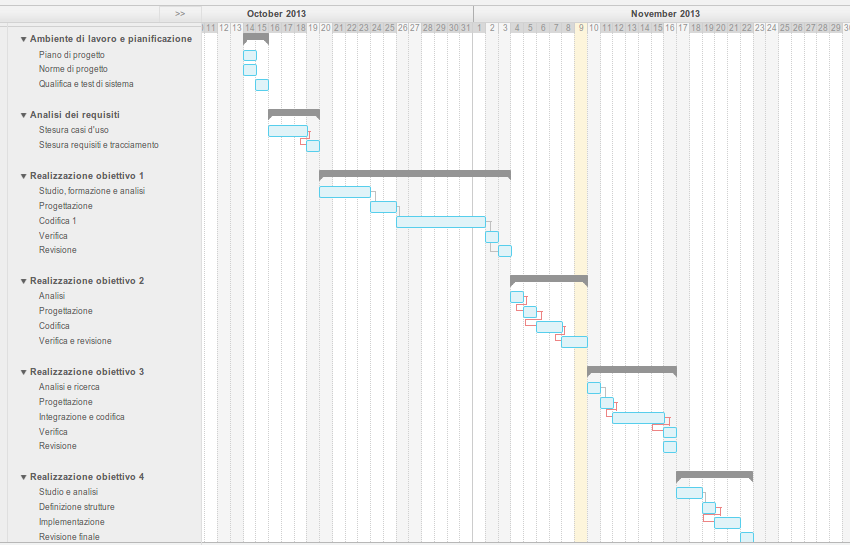
\includegraphics[width=1.0\textwidth]{./images/pianificazione.png}
\caption{diagramma di Gantt che descrive la pianificazione}
\label{fig:pianificazione}
\end{figure}







\clearpage

\section{Analisi dei Requisiti} \label{sec:analisi}

\subsection{Casi d'uso} \label{sec:casiduso}
In questa sezione verranno elencati i casi d'uso del sistema che è oggetto dello stage. Dato che il sistema è stato pensato per rispondere solo all'intervento di un utente che si occupa di amministrazione e installazione l'unico attore che prenderemo in considerazione è \textbf{utente}. Per ogni caso d'uso verranno riportate:
\begin{enumerate}
\item DESCRIZIONE: contenuto del caso d'uso
\item FLUSSO PRINCIPALE DEGLI EVENTI
\item PRECONDIZIONI: asserzioni che sono valide prima dell'effettiva esecuzione del caso d'uso
\item POSTCONDIZIONI: asserzioni che sono valide dopo l'esecuzione del caso d'uso
\item SCENARI ALTERNATIVI: eventuali scenari alternativi che differiscono dal normale flusso del caso d'uso
\end{enumerate}
Ogni caso d'uso ha un identificativo stile UC\textit{n} dove n indica una posizione gerarchica.
Ogni caso d'uso è posizionato all'interno della gerarchia che parte dal caso d'uso più generale UC0 (radice dell'albero). Per ogni caso d'uso figlio valgono le precondizioni del padre.
\subsubsection{UC0: Scenario principale} \label{sec:UC0}
\begin{description}
\item[\em{descrizione }]L'utente ha avviato il sistema il quale è pronto a rispondere agli eventi. L'utente può scegliere di accedere alla calibrazione delle telecamere, accedere alla loro configurazione, oppure generare le statistiche a partire dai dati di tracking attualmente presenti nel sistema (figura ~\ref{fig:uc0})
\item[\em{flusso principale degli eventi }] \mbox{}
 \begin{enumerate}
\item L'utente può calibrare le telecamere (\hyperref[sec:uc1]{UC1}) 
\item L'utente può configurare le telecamere (\hyperref[sec:uc2]{UC2})
\item L'utente può generare e visualizzare le statistiche (\hyperref[sec:uc3]{UC3})
\end{enumerate}
\item[\em{precondizione }] Il sistema è avviato e funzionante
\end{description}

\begin{figure}[htpb] 

\centering 

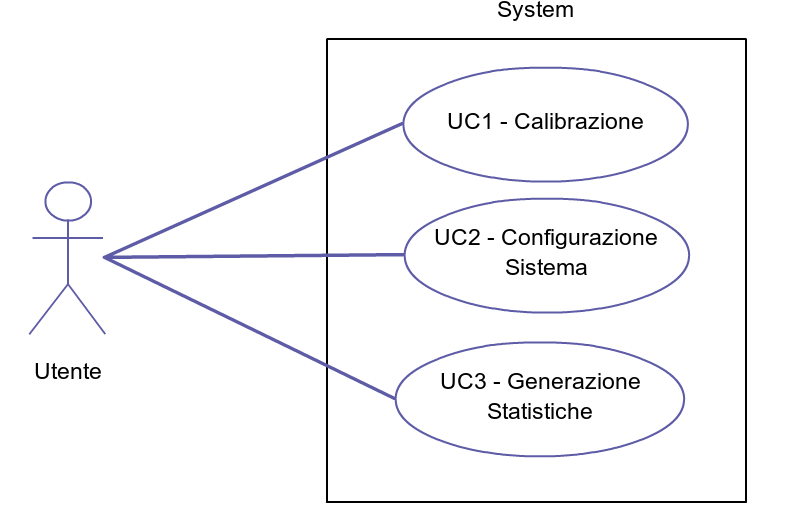
\includegraphics[scale=0.4]{./images/uc0.png} 

\caption{UC0 - Scenario principale} 

\label{fig:uc0}

\end{figure} 

\subsubsection{UC1: Calibrazione telecamere} \label{sec:UC1}
\begin{description}
\item[\em{descrizione }]L'utente può iniziare la calibrazione delle telecamere, oppure può visualizzare un video \textit{undistorted} che usa i parametri di calibrazione per correggere i frame prodotti dal video. (figura ~\ref{fig:uc1})
\item[\em{flusso principale degli eventi }] \mbox{}
 \begin{enumerate}
\item L'utente può iniziare la calibrazione (\hyperref[sec:uc1.1]{UC1.1}) 
\item L'utente può visualizzare il video corretto con i parametri di calibrazione (\hyperref[sec:uc1.2]{UC1.2})
\end{enumerate}
\item[\em{precondizione }] Il sistema è avviato e funzionante
\end{description}

\begin{figure}[htpb] 

\centering 

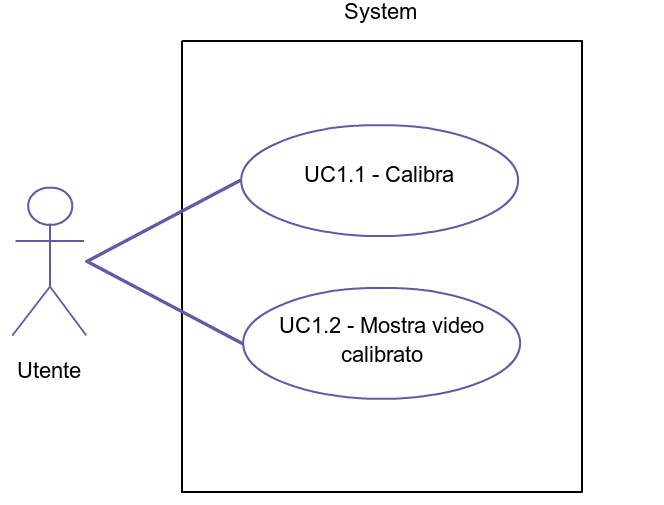
\includegraphics[scale=0.4]{./images/uc1.png} 

\caption{UC1 - Calibrazione telecamere} 

\label{fig:uc1}

\end{figure} 

\subsubsection{UC1.1: Calibra} \label{sec:UC1.1}
\begin{description}
\item[\em{descrizione }]L'utente sta selezionando le opzioni per la calibrazione delle telecamere. Può selezionare: numero di immagini da utilizzare nella calibrazione, il frame step indirizzo IP nella rete della camera da calibrare, e poi iniziare l'effettiva calibrazione.  (figura ~\ref{fig:uc1.1})
\item[\em{flusso principale degli eventi }] \mbox{}
 \begin{enumerate}
\item L'utente seleziona il numero di immagini da utilizzare (\hyperref[sec:uc1.1.1]{UC1.1.1})
\item L'utente seleziona il frame step (\hyperref[sec:uc1.1.2]{UC1.1.2})
\item L'utente seleziona l'indirizzo della camera da calibrare (\hyperref[sec:uc1.1.3]{UC1.1.3})
\item L'utente avvia la calibrazione calibrare (\hyperref[sec:uc1.1.4]{UC1.1.4})
\end{enumerate}
\item[\em{postcondizione }] I file che contengono i file di calibrazione della telecamera (distortion e instrinsics) sono stati generati e salvati nel file system
\item[\em{scenari alternativi }] \mbox{}

  \begin{enumerate}
\item L'utente interrompe la procedura, il sistema torna in attesa di eventi
\item La procedura di calibrazione fallisce, il sistema segnala l'errore e torna in attesa di eventi
\end{enumerate}
\end{description}

\begin{figure}[htpb] 

\centering 

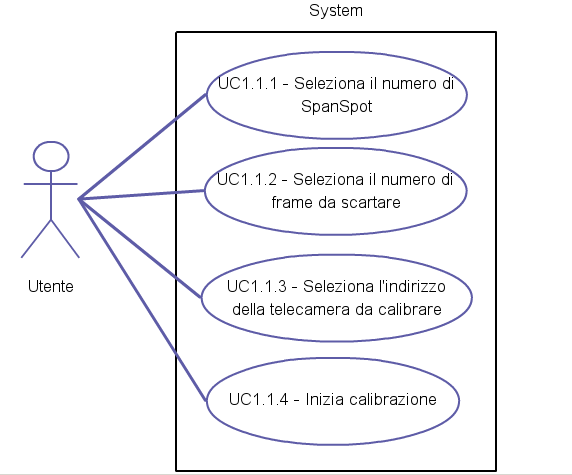
\includegraphics[scale=0.4]{./images/uc11.png} 

\caption{UC1.1 - Calibra} 

\label{fig:uc1.1}

\end{figure} 

\subsubsection{UC1.1.1: Seleziona il numero di immagini da utilizzare} \label{sec:UC1.1.1}
\begin{description}
\item[\em{descrizione }]L'utente seleziona il numero di immagini da utilizzare per la calibrazione
\item[\em{postcondizione }] Il sistema conosce il numero di immagini da utilizzare da utilizzare nella calibrazione
\item[\em{scenari alternativi }] \mbox{}

  \begin{enumerate}
\item L'utente interrompe la procedura, il sistema ritorna in attesa di eventi
\end{enumerate}
\end{description}

\subsubsection{UC1.1.2: Seleziona il frame step} \label{sec:UC1.1.2}
\begin{description}
\item[\em{descrizione }]L'utente seleziona il frame step per la calibrazione
\item[\em{precondizione }] L'utente ha già selezionato il numero immagini da utilizzare
\item[\em{postcondizione }] Il sistema conosce il frame step per la calibrazione
\item[\em{scenari alternativi }] \mbox{}

  \begin{enumerate}
\item L'utente interrompe la procedura, il sistema ritorna in attesa di eventi
\end{enumerate}
\end{description}

\subsubsection{UC1.1.3: Inserisce l'indirizzo della telecamera da calibrare} \label{sec:UC1.1.3}
\begin{description}
\item[\em{descrizione }]L'utente inserisce l'indirizzo della telecamera da calibrare
\item[\em{precondizione }] L'utente ha già selezionato il numero immagini da utilizzare e il frame step per la calibrazione
\item[\em{postcondizione }] Il sistema conosce l'indirizzo della telecamera da calibrare
\item[\em{scenari alternativi }] \mbox{}

  \begin{enumerate}
\item L'utente interrompe la procedura, il sistema ritorna in attesa di eventi
\end{enumerate}
\end{description}

\subsubsection{UC1.1.4: Inizia calibrazione} \label{sec:UC1.1.4}
\begin{description}
\item[\em{descrizione }]L'utente inizia la calibrazione effettiva
\item[\em{precondizione }] L'utente ha già selezionato le opzioni di calibrazione (UC1.1.1 - UC1.1.2 - UC1.1.3), il sistema quindi conosce i parametri da utilizzare
\item[\em{postcondizione }] Il sistema genera i file di calibrazione intrinsics e distortion e li salva nel file system
\item[\em{scenari alternativi }] \mbox{}

  \begin{enumerate}
\item La calibrazione non termina con successo quindi l'operazione viene interrotta e l'errore segnalato. Il sistema ritorna in attesa di eventi
\end{enumerate}
\end{description}

\subsubsection{UC1.2: Mostra video calibrato} \label{sec:UC1.2}
\begin{description}
\item[\em{descrizione }]L'utente visualizza il video corretto con i valori di calibrazione
\item[\em{precondizione }] L'utente ha già effettuato con successo la generazione dei file di calibrazione che sono presenti nel sistema
\end{description}

\subsubsection{UC2: Configurazione telecamere} \label{sec:UC2}
\begin{description}
\item[\em{descrizione }]L'utente può impostare le opzioni di configurazione delle telecamere, aggiungendone di nuove, rimuovendole, modificandole. Può inoltre ottenere i file necessari alla configurazione, convertendo un file .DXF in .PNG, salvando un frame dalla telecamera, o calcolare la \textit{homography matrix} (figura ~\ref{fig:uc2})
\item[\em{flusso principale degli eventi }] \mbox{}
 \begin{enumerate}
\item L'utente inserisce una nuova telecamera nel sistema (\hyperref[sec:uc2.1]{UC2.1})
\item L'utente rimuove una telecamera esistente (\hyperref[sec:uc2.2]{UC2.2})
\item L'utente modifica la configurazione di una telecamera (\hyperref[sec:uc2.3]{UC2.3})
\item L'utente cattura e salva un frame della telecamera (\hyperref[sec:uc2.4]{UC2.4})
\item L'utente converte un file .DXF in .PNG (\hyperref[sec:uc2.5]{UC2.5})
\item L'utente calcola la matrice omografica relativa ad una telecamera (\hyperref[sec:uc2.6]{UC2.6})
\item L'utente seleziona una telecamera (\hyperref[sec:uc2.7]{UC2.7})
\end{enumerate}
\item[\em{precondizione }] Il sistema è avviato e funzionante.
\end{description}

\begin{figure}[htpb] 

\centering 

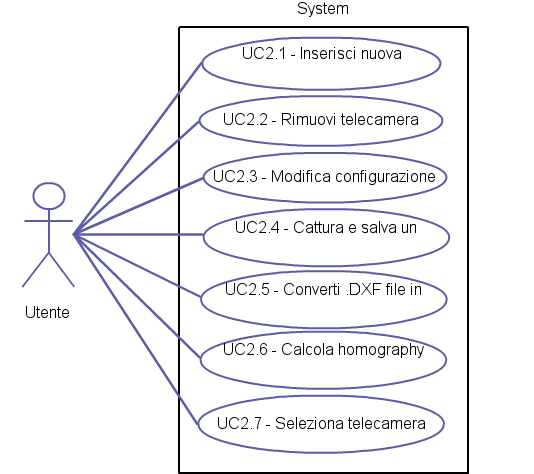
\includegraphics[scale=0.4]{./images/uc2.png} 

\caption{UC2 - Configurazione telecamere} 

\label{fig:uc2}

\end{figure} 

\subsubsection{UC2.1: Inserisci nuova} \label{sec:UC2.1}
\begin{description}
\item[\em{descrizione }]L'utente inserisce il nome della nuova telecamera
\item[\em{postcondizione }] Il sistema ha inserito la nuova telecamera nel database
\item[\em{scenari alternativi }] \mbox{}

  \begin{enumerate}
\item Il nome inserito non è valido, il sistema interrompe l'operazione e torna in attesa di eventi.
\end{enumerate}
\end{description}

\subsubsection{UC2.2: Rimuovi telecamera} \label{sec:UC2.2}
\begin{description}
\item[\em{descrizione }]L'utente rimuove la telecamera selezionata
\item[\em{precondizione }] L'utente ha selezionato una telecamera tra quelle esistenti
\item[\em{postcondizione }] Il sistema ha rimosso la telecamera dal database
\end{description}

\subsubsection{UC2.3: Modifica configurazione} \label{sec:UC2.3}
\begin{description}
\item[\em{descrizione }]L'utente ha selezionato una telecamera e ne modifica le opzioni di configurazione, quali: file distortion, intrinsics, valore dell'altezza del frame, valore della larghezza del frame, percorso del file contentente la \textit{homography matrix} (figura ~\ref{fig:uc2.3}).
\item[\em{flusso principale degli eventi }] \mbox{}
 \begin{enumerate}
\item L'utente modifica il percorso del file di calibrazione \textit{distortion} (\hyperref[sec:uc2.3.1]{UC2.3.1})
\item L'utente modifica il percorso del file di calibrazione \textit{intrinsics} (\hyperref[sec:uc2.3.2]{UC2.3.2})
\item L'utente modifica il valore dell'altezza del frame (\hyperref[sec:uc2.3.3]{UC2.3.3})
\item L'utente modifica il valore della larghezza del frame (\hyperref[sec:uc2.3.4]{UC2.3.4})
\item L'utente modifica il percorso del file di configurazione contenente la \textit{homography matrix} (\hyperref[sec:uc2.3.5]{UC2.3.5})
\end{enumerate}
\item[\em{precondizione }] L'utente ha selezionato una telecamera tra quelle esistenti
\item[\em{scenari alternativi }] \mbox{}

  \begin{enumerate}
\item L'utente interrompe la modifica, il sistema ritorna in attesa di eventi
\end{enumerate}
\end{description}

\begin{figure}[htpb] 

\centering 

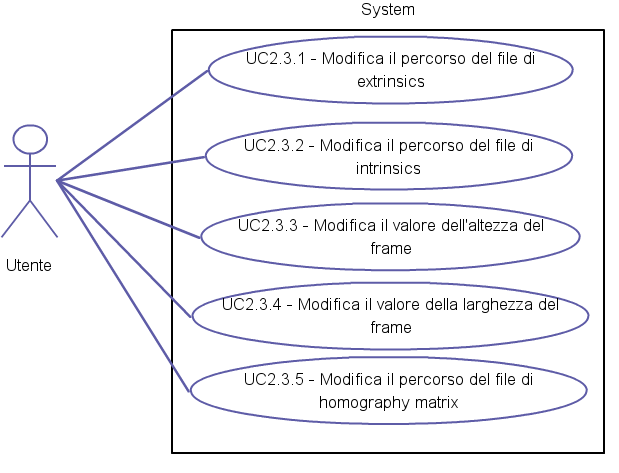
\includegraphics[scale=0.4]{./images/uc23.png} 

\caption{UC2.3 - Modifica configurazione} 

\label{fig:uc2.3}

\end{figure} 

\subsubsection{UC2.3.1: Modifica il percorso del file di distortion} \label{sec:UC2.3.1}
\begin{description}
\item[\em{descrizione }]L'utente seleziona un file nel file system che contiene i valori \textit{distortion} di calibrazione.
\item[\em{postcondizione }] Il sistema ha modificato il corrispondente valore della telecamera nel database
\item[\em{scenari alternativi }] \mbox{}

  \begin{enumerate}
\item L'utente interrompe la selezione del file, il sistema ritorna in attesa di eventi
\end{enumerate}
\end{description}

\subsubsection{UC2.3.2: Modifica il percorso del file di intrinsics} \label{sec:UC2.3.2}
\begin{description}
\item[\em{descrizione }]L'utente seleziona un file nel file system che contiene i valori \textit{intrinsics} di calibrazione.
\item[\em{postcondizione }] Il sistema ha modificato il corrispondente valore della telecamera nel database
\item[\em{scenari alternativi }] \mbox{}

  \begin{enumerate}
\item L'utente interrompe la selezione del file, il sistema ritorna in attesa di eventi
\end{enumerate}
\end{description}

\subsubsection{UC2.3.3: Modifica il valore dell'altezza del frame} \label{sec:UC2.3.3}
\begin{description}
\item[\em{descrizione }]L'utente seleziona un valore per l'altezza del frame della telecamera.
\item[\em{postcondizione }] Il sistema ha modificato il corrispondente valore della telecamera nel database
\end{description}

\subsubsection{UC2.3.4: Modifica il valore della larghezza del frame} \label{sec:UC2.3.4}
\begin{description}
\item[\em{descrizione }]L'utente seleziona un valore per la larghezza del frame della telecamera.
\item[\em{postcondizione }] Il sistema ha modificato il corrispondente valore della telecamera nel database
\end{description}

\subsubsection{UC2.3.5: Modifica il percorso del file di homography matrix} \label{sec:UC2.3.5}
\begin{description}
\item[\em{descrizione }]L'utente seleziona un file nel file system che contiene i valori che descrivono la  \textit{homography matrix} utilizzata per la traduzione delle coordinate.
\item[\em{postcondizione }] Il sistema ha modificato il corrispondente valore della telecamera nel database
\item[\em{scenari alternativi }] \mbox{}

  \begin{enumerate}
\item L'utente interrompe la selezione del file, il sistema ritorna in attesa di eventi
\end{enumerate}
\end{description}

\subsubsection{UC2.4: Cattura e salva un frame della telecamera} \label{sec:UC2.4}
\begin{description}
\item[\em{descrizione }]L'utente indica al sistema di attivare la telecamera selezionata, catturare un frame e salvarlo.
\item[\em{precondizione }] L'utente ha selezionato una telecamera tra quelle esistenti
\item[\em{postcondizione }] Il frame della telecamera selezionata è stato salvato nel file system
\item[\em{scenari alternativi }] \mbox{}

  \begin{enumerate}
\item La telecamera non è raggiungibile, il sistema interrompe l'operazione segnala l'errore e ritorna in attesa di eventi
\end{enumerate}
\end{description}

\subsubsection{UC2.5: Converti .DXF file in .PNG} \label{sec:UC2.5}
\begin{description}
\item[\em{descrizione }]L'utente seleziona nel file system un file .DXF da convertire in formato .PNG 
    
\item[\em{postcondizione }] Il file selezionato è stato convertito in un immagine che riproduce il contenuto del .DXF
\end{description}

\subsubsection{UC2.6: Calcola homography matrix} \label{sec:UC2.6}
\begin{description}
\item[\em{descrizione }]L'utente calcola la homography matrix per una particolare telecamera configurata.
\item[\em{postcondizione }] Il file che contiene la \textit{homography matrix} è stato calcolato e salvato nel file system
\end{description}

\subsubsection{UC2.7: Seleziona telecamera} \label{sec:UC2.7}
\begin{description}
\item[\em{descrizione }]L'utente seleziona una telecamera tra la lista di telecamere presenti nel sistema
\item[\em{postcondizione }] La telecamera indicata diventa selezionata e quindi \textbf{attiva}
\end{description}

\subsubsection{UC3: Generazione statistiche} \label{sec:UC3}
\begin{description}
\item[\em{descrizione }]L'utente può visualizzare le statistiche relative ai dati presenti nel sistema. Può effettuare la conversione dei dati \textit{raw}, visualizzare l'\textit{heatmap}, o le statistiche (figura ~\ref{fig:uc3})
\item[\em{flusso principale degli eventi }] \mbox{}
 \begin{enumerate}
\item L'utente seleziona la trasformazione dei dati di tracciamento presenti nel sistema (\hyperref[sec:uc3.1]{UC3.1})
\item L'utente seleziona la generazione dell'heatmap (\hyperref[sec:uc3.2]{UC3.2})
\item L'utente seleziona la generazione delle statistiche (\hyperref[sec:uc3.3]{UC3.3})
\end{enumerate}
\item[\em{precondizione }] Il sistema è avviato e funzionante.
\end{description}

\begin{figure}[htpb] 

\centering 

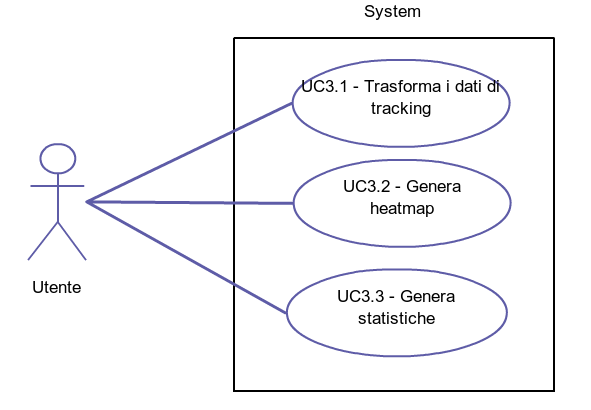
\includegraphics[scale=0.4]{./images/uc3.png} 

\caption{UC3 - Generazione statistiche} 

\label{fig:uc3}

\end{figure} 

\subsubsection{UC3.1: Trasforma i dati di tracking} \label{sec:UC3.1}
\begin{description}
\item[\em{descrizione }]L'utente indica al sistema di eseguire la trasformazione dei dati \textit{raw} di tracking
\item[\em{postcondizione }] Il sistema ha trasformato i dati presenti nel database ed ha salvato i dati trasformati.
\item[\em{scenari alternativi }] \mbox{}

  \begin{enumerate}
\item La trasformazione fallisce, il sistema segnala l'errore e torna in attesa di eventi
\end{enumerate}
\end{description}

\subsubsection{UC3.2: Genera heatmap} \label{sec:UC3.2}
\begin{description}
\item[\em{descrizione }]L'utente indica al sistema di generare l'heatmap con la rappresentazione grafica dei dati di tracking
\item[\em{postcondizione }] Il sistema elabora i dati presenti nel database generando l'heatmap e salvandola nel file system.
\item[\em{scenari alternativi }] \mbox{}

  \begin{enumerate}
\item La generazione fallisce, il sistema segnala l'errore e torna nello stato di attesa.
\end{enumerate}
\end{description}

\subsubsection{UC3.3: Genera statistiche} \label{sec:UC3.3}
\begin{description}
\item[\em{descrizione }]L'utente indica al sistema di generare le statistiche relative ai dati presenti
\item[\em{postcondizione }] Il sistema ha generato le statistiche e le ha salvate nel database
\item[\em{scenari alternativi }] \mbox{}

  \begin{enumerate}
\item La generazione fallisce, il sistema segnala l'errore e torna nello stato di attesa.
\end{enumerate}
\end{description}


\newpage
\subsection{Requisiti} \label{sec:req}
In questa sezione verranno elencati i requisiti software che sono emersi dai casi d'uso individuati e dalle riunioni informative con i leader dello sviluppo. Per chiarezza si è cercato di tenere un rapporto 1:1 tra casi d'uso e requisiti.
 \\ \\Nell'esposizione si userà la seguente convenzione: se un requisito padre ha figli con tipologia diversa tra di loro, il requisito padre assumerà la tipologia più vincolante tra quelle dei figli (esempio: se ci sono 2 figli, uno obbligatorio ed uno desiderabile il padre sarà qualificato come obbligatorio).

\subsubsection{Requisiti funzionali} \label{sec:reqfun}
\begin{center}
    \begin{longtable}{ | l | p{5cm} | c | p{1.5cm} |}
    \caption{Tabella requisiti funzionali} \\
    \hline 
    \textbf{Codice} & \textbf{Descrizione} & \textbf{Tipologia} & \textbf{Fonte} \\ \hline
\endfirsthead
\multicolumn{4}{c}%
{\tablename\ \thetable\ -- \textit{Continued from previous page}} \\
\hline
\textbf{Codice} & \textbf{Descrizione} & \textbf{Tipologia} & \textbf{Fonte} \\
\hline
\endhead
\hline \multicolumn{4}{r}{\textit{Continued on next page}} \\
\endfoot
\hline
\endlastfoot
    RF1 & Il sistema deve permettere all'utente di eseguire la calibrazione delle telecamere & Obbligatorio & UC1
    \\ \hline
    RF1.1 & Il sistema deve permettere all'utente di impostare le opzioni di calibrazione & Obbligatorio & UC1  UC1.1
    \\ \hline
    RF1.1.1 & Il sistema deve permettere all'utente di selezionare il numero di span spot per la calibrazione & Obbligatorio & UC1  UC1.1 UC1.1.1
    \\ \hline
    RF1.1.2 & Il sistema deve permettere all'utente di selezionare il numero di span spot per la calibrazione & Obbligatorio & UC1  UC1.1 UC1.1.2
    \\ \hline
    RF1.1.3 & Il sistema deve permettere all'utente di selezionare l'indirizzo identificativo della telecamera & Obbligatorio & UC1.1 UC1.1.3
    \\ \hline
    RF1.1.4 & Il sistema deve eseguire la calibrazione delle telecamere con le opzioni impostate & Obbligatorio & UC1.1 UC1.1.4
    \\ \hline
    RF1.2 & Il sistema deve permettere all'utente di visualizzare un video che utilizza i parametri di calibrazione per correggere i frame & Desiderabile & UC1  UC1.2
    \\ \hline
    RF2 & Il sistema deve permettere all'utente di configurare le telecamere & Obbligatorio & UC2
    \\ \hline
    RF2.1 & Il sistema deve permettere all'utente di inserire una nuova telecamera & Obbligatorio & UC2 UC2.1
    \\ \hline
    RF2.2 & Il sistema deve permettere all'utente di rimuovere una telecamera & Obbligatorio & UC2 UC2.2
    \\ \hline
    RF2.3 & Il sistema deve permettere all'utente di modificare e salvare in maniera persistente la configurazione di una telecamera esistente & Obbligatorio & UC2 UC2.3
    \\ \hline
    RF2.3.1 & Il sistema deve permettere all'utente di modificare il file di extrinsics di calibrazione di una telecamera & Desiderabile & UC2 UC2.3 UC2.3.1
    \\ \hline
    RF2.3.2 & Il sistema deve permettere all'utente di modificare il file di intrinsics di calibrazione di una telecamera & Desiderabile & UC2 UC2.3 UC2.3.2
    \\ \hline
    RF2.3.3 & Il sistema deve permettere all'utente di modificare il valore dell'altezza del frame utilizzato per una telecamera & Obbligatorio & UC2 UC2.3 UC2.3.3
    \\ \hline
    RF2.3.4 & Il sistema deve permettere all'utente di modificare il valore della larghezza del frame utilizzato per una telecamera & Obbligatorio & UC2 UC2.3 UC2.3.4
    \\ \hline
    RF2.3.5 & Il sistema deve permettere all'utente di modificare il file contenente la homography matrix utilizzata per la traduzione delle coordinate di tracking relative ad una telecamera & Obbligatorio & UC2 UC2.3 UC2.3.5
    \\ \hline
    RF2.4 & Il sistema deve permettere di salvare un frame preso dal video stream della telecamera & Obbligatorio & UC2 UC2.4
    \\ \hline
    RF2.5 & Il sistema deve permettere di convertire un file .DXF in un file .PNG che riproduce graficamente l'immagine contenuta nel file originale & Obbligatorio & UC2 UC2.5
    \\ \hline
    RF2.6 & Il sistema deve permettere di calcolare la homography matrix utilizzata per la traduzione delle coordinate di tracking relative ad una telecamera & Obbligatorio & UC2 UC2.6
    \\ \hline
    RF2.7 & Il sistema deve permettere di selezionare una telecamera per la modifica & Obbligatorio & UC2 UC2.7
    \\ \hline
    RF3 & Il sistema deve permettere all'utente di generare delle statistiche a partire dai dati di tracking attualmente presenti & Obbligatorio & UC3
    \\ \hline
    RF3.1 & Il sistema deve permettere di trasformare i dati di tracking in coordinate di posizione all'interno di un immagine .PNG che descrive la planimetria del locale, e di salvare tali informazioni in maniera persistente & Obbligatorio & UC3 UC3.1
    \\ \hline
    RF3.2 & Il sistema deve permettere di generare un heatmap grafica che fornisca una rappresentazione grafica dei dati di tracking & Obbligatorio & UC3 UC3.2
   \\ \hline
    RF3.3 & Il sistema deve permettere di generare delle statistiche numeriche a partire dai dati di tracking e di salvarle in maniera persistente & Facoltativo & UC3 UC3.1
    
    \\ \hline
    RF3.3.1 & Il sistema deve permettere di generare la statistica di \textit{Dwell Time} & Facoltativo & UC3 UC3.1
    
    \\ \hline
    RF3.3.2 & Il sistema deve permettere di generare la statistica di \textit{Counting} & Facoltativo & UC3 UC3.1
    
    \\ \hline
    RF3.3.3 & Il sistema deve permettere di generare la statistica di \textit{Waiting Line} & Facoltativo & UC3 UC3.1

    \end{longtable}
\end{center}


\subsubsection{Requisiti di vincolo}\label{sec:reqvin}
\begin{center}
    \begin{longtable}{ | l | p{5cm} | c | p{1.5cm} |}
    \caption{Tabella requisiti di vincolo} \\
    \hline 
    \textbf{Codice} & \textbf{Descrizione} & \textbf{Tipologia} & \textbf{Fonte} \\ \hline
\endfirsthead
\multicolumn{4}{c}%
{\tablename\ \thetable\ -- \textit{Continued from previous page}} \\
\hline
\textbf{Codice} & \textbf{Descrizione} & \textbf{Tipologia} & \textbf{Fonte} \\
\hline
\endhead
\hline \multicolumn{4}{r}{\textit{Continued on next page}} \\
\endfoot
\hline
\endlastfoot
    RV1 & Il sistema dev'essere strutturato secondo un'architettura 3-tier & Obbligatorio & Capitolato
    \\ \hline
    RV2 & Il sistema deve funzionare in ambiente Linux & Obbligatorio & Capitolato
    \\ \hline
    RV3 & Il sistema deve funzionare in ambiente Windows & Facoltativo & Capitolato
    \\ \hline
    RV4 & Il sistema deve funzionare in ambiente Mac OS X & Desiderabile & Capitolato
    \\ \hline
    RV5 & Il sistema utilizzerà come strumento di build CMake, verranno quindi forniti i relativi file & Obbligatorio & Capitolato
    \\ \hline
\end{longtable}
\end{center}

    
\subsubsection{Requisiti di qualità}\label{sec:reqqua}
\begin{center}
    \begin{longtable}{ | l | p{5cm} | c | p{1.5cm} |}
    \caption{Tabella requisiti di qualità} \\
    \hline 
    \textbf{Codice} & \textbf{Descrizione} & \textbf{Tipologia} & \textbf{Fonte} \\ \hline
\endfirsthead
\multicolumn{4}{c}%
{\tablename\ \thetable\ -- \textit{Continued from previous page}} \\
\hline
\textbf{Codice} & \textbf{Descrizione} & \textbf{Tipologia} & \textbf{Fonte} \\
\hline
\endhead
\hline \multicolumn{4}{r}{\textit{Continued on next page}} \\
\endfoot
\hline
\endlastfoot
    RQ1 & Deve essere prodotta documentazione del codice sorgente del software & Obbligatorio & Interno
    \\ \hline
    RQ2 & Il sistema deve garantire la massima indipendenza tra le funzionalità & Desiderabile & Capitolato
    \\ \hline
\end{longtable}
\end{center}


 
 
\newpage
\subsubsection{Tracciamento requisiti}\label{sec:tracciamento}
\begin{center}
{\renewcommand{\arraystretch}{1.5} 
    \begin{longtable}{ | c | p{1.5cm} |}
    \caption{Tabella tracciamento requisiti - casi d'uso} \\
    \hline 
    \textbf{Fonte} & \textbf{Requisiti}  \\ \hline
\endfirsthead
\multicolumn{2}{c}% 

{\tablename\ \thetable\ -- \textit{Continued from previous page}} \\
\hline
 \textbf{Fonte} & \textbf{Requisiti} \\
\hline
\endhead
\hline \multicolumn{2}{r}{\textit{Continued on next page}} \\
\endfoot
\hline
\endlastfoot 
Interno & RF2.5 \\ \hline 
Interno & RF3.1 \\ \hline 
Interno & RQ1 \\ \hline 
Capitolato & RQ2 \\ \hline 
Capitolato & RV1 \\ \hline 
Capitolato & RV2 \\ \hline 
Capitolato & RV3 \\ \hline 
Capitolato & RV4 \\ \hline 
Capitolato & RV5 \\ \hline 
UC1 Calibrazione telecamere & RF1 \\ \hline 
UC1.1 Calibra & RF1.1 \\ \hline 
UC1.1.1 Seleziona il numero di immagini da utilizzare & RF1.1.1 \\ \hline 
UC1.1.2 Seleziona il frame step & RF1.1.2 \\ \hline 
UC1.1.3 Inserisce l'indirizzo della telecamera da calibrare & RF1.1.3 \\ \hline 
UC1.1.4 Inizia calibrazione & RF1.1.4 \\ \hline 
UC1.2 Mostra video calibrato & RF1.2 \\ \hline 
UC2 Configurazione telecamere & RF2 \\ \hline 
UC2.1 Inserisci nuova & RF2.1 \\ \hline 
UC2.2 Rimuovi telecamera & RF2.2 \\ \hline 
UC2.3 Modifica configurazione & RF2.3 \\ \hline 
UC2.3.1 Modifica il percorso del file di distortion & RF2.3.1 \\ \hline 
UC2.3.2 Modifica il percorso del file di intrinsics & RF2.3.2 \\ \hline 
UC2.3.3 Modifica il valore dell'altezza del frame & RF2.3.3 \\ \hline 
UC2.3.4 Modifica il valore della larghezza del frame & RF2.3.4 \\ \hline 
UC2.3.5 Modifica il percorso del file di homography matrix & RF2.3.5 \\ \hline 
UC2.4 Cattura e salva un frame della telecamera & RF2.4 \\ \hline 
UC2.6 Calcola homography matrix & RF2.6 \\ \hline 
UC2.7 Seleziona telecamera & RF2.7 \\ \hline 
UC3 Generazione statistiche & RF3 \\ \hline 
UC3.2 Genera heatmap & RF3.2 \\ \hline 
UC3.3 Genera statistiche & RF3.3 \\ \hline 
UC3.3 Genera statistiche & RF3.3.1 \\ \hline 
UC3.3 Genera statistiche & RF3.3.2 \\ \hline 
UC3.3 Genera statistiche & RF3.3.3 \\ \hline 
\end{longtable} }
\end{center} 

\newpage
{\section{Tecnologie Utilizzate} \label{sec:tecnologie}
In questa sezione vengono brevemente introdotte le più interessanti tecnologie utilizzate nello sviluppo dell'applicazione, e vengono esposte le motivazioni che hanno portato alla scelta di tali tecnologie.
\subsection{Librerie}
\subsubsection{OpenCV}
OpenCV è una libreria open source il cui obiettivo è quello di fornire un'API per il supporto al real-time computer vision. Essa è sviluppata da Intel ed attualmente manutenuta da \textit{itseez} (\url{http://itseez.com/}). OpenCV è rilasciata con licenza BSD open source, ed è libera per quanto riguarda l'utilizzo accademico e commercial. E' scritta in C/C++ e fornisce le interfacce per diversi linguaggi: C++, C, Python, MATLAB e Java. \\ \\
Questa libreria è cross platform e supporta i più comuni sistemi: Windows, Linux, Mac OS, iOS e Android. \\ 
OpenCV viene ufficialmente rilasciata nel 1999, attualmente l'ultima versione stabile ufficiale è la 2.4.6. \\
OpenCV è una libreria molto ampia e completa, è attualmente utilizzata in diverse applicazioni complesse (molte che riguardano la \textit{video surveillance}), inoltre ha alle spalle anni di sviluppo e una comunità di utenti molto vasta. \\
L'intero sistema che l'azienda Pathflow vuole realizzare è basato su tale libreria, nelle specifiche del progetto di stage è stato specificato che essa verrà utilizzata per quanto riguarda le funzioni relative alla \textit{computer vision}. 

\subsubsection{Qt}
Dato che il progetto prevede la realizzazione di una minimale interfaccia grafica si è scelto di utilizzare il framework Qt. \\
Le valutazioni che hanno portato a tale scelta, sono le seguenti:
\begin{itemize}
\item \textbf{Portabilità:} Qt è una libreria cross platform. Nelle specifiche del progetto è emerso che sarebbe stato fondamentale che il software fosse portabile. Altra caratteristica che ha influito è che Qt offre un buon supporto per effettuare manipolazioni grafiche e disegno, e dopo una ricerca si è rivelata la migliore alternativa tra le librerie disponibili (sono state valutate altre librerie alternative per il solo disegno, ma esse si sono rivelate meno complete e spesso scarsamente documentate).
\item \textbf{Licenza: } Qt è infatti disponibile con licenza  GNU LGPL v2.1 ed è quindi possibile utilizzarlo senza che sia necessario rilasciare il sorgente del prodotto.
\end{itemize}
\subsubsection{MySQL wrapped}
Per facilitare il \textit{system management} è stato scelto di usare una semplice libreria che fornisce le funzionalità di \textit{Object Relational Mapping} per un database di tipo MySQL. Tra le varie opzioni si è scelto di usare MySQL Wrapped, molto semplice e leggera. Essa inoltre fornisce un tool di generazione codice C++ a partire dall'output del comando \textit{mysqldump}. In tale modo si è potuto progettare prima lo schema del database e in seguito creare le rispettive classi con lo script \textit{sql2class}. MySQL Wrapped crea un ulteriore livello di astrazione a partire dall'API di connessione in C fornita da MySQL.

\subsubsection{dxflib}
Il file .DXF è un file di output di programmi di grafica vettoriali quali AutoCAD. Esso contiene al suo interno delle entità che definiscono gli elementi che descrivono un immagine (generalmente 2D). \\
Il formato dei file .DXF è noto e ben documentato nei manuali forniti da AutoCAD.
Per le funzionalità di parsing del file .DXF si è scelto di utilizzare dxflib: una libreria in C++ open source. Essa si occupa della lettura del file e definisce delle interfacce che possono essere ridefinite per ottenere il comportamento desiderato. I dettagli verranno trattati meglio in seguito.

\subsection{MySQL}
Il database scelto per il salvataggio dei dati è MySQL. Le motivazioni di tale scelta sono nuovamente la necessità di avere un \textit{DBMS} cross platform e open source. In fase di studio sono state valutate anche altre alternative, che vengono qui brevemente elencate con i relativi difetti che hanno comportato la preferenza per MySQL:
\begin{itemize}

	\item \textbf{memsql} è un database che nasce per fornire supporto al real-time analytics. Viene preso in esame per le sue caratteristiche di velocità che renderebbero l'elaborazione del grande carico di dati molto veloce. Tali caratteristiche sono dovute al fatto che memsql è un database che risiede in memoria (RAM), e che non esegue direttamente le query, ma le converte in codice C++ (con GCC) e poi esegue il codice oggetto. Sebbene tali caratteristiche sono molto favorevoli si è preferito non utilizzare memsql in quanto essendo un progetto relativamente nuovo non ha ancora un supporto completo delle caratteristiche di un database relazionale e in quanto c'era la necessità di appoggiarsi su una soluzione solida che avrebbe dato certezze nel tempo.
	
	\item \textbf{mongoDB} è un database di tipo non relazionale (\textit{document-oriented}). Esso si basa su documenti stile JSON con schemi dinamici. Anche mongoDB è stato preso in considerazione per le sue caratteristiche di velocità che avrebbero fatto comodo per l'elaborazione dei moltissimi dati di tracciamento. Si è però preferito basarsi su un database di tipo relazionale in quanto la tipologia di dati che andava memorizzata era strettamente di tale tipo.
\end{itemize}



\subsection{CMake}
CMake è un sistema di build cross platform e open source. Nasce per fornire un sistema di management del processo di build del software. Per ottenere ciò CMake utilizza dei metodi che non dipendono dal tipo di compilatore presente nel sistema operativo, ma da alcuni file di configurazione autonomi. CMake genera dei makefiles che possono in seguito essere eseguiti con il comando di make relativo all'ambiente utilizzato (\textit{make} per Linux, \textit{nmake} per Visual Studio etc). CMake supporta sia build di tipo \textit{in-place} che \textit{out-of-place}, supporta inoltre linking di tipo statico e dinamico. \\ \\
Per il suo utilizzo è sufficiente creare dei file denominati CMakeLists.txt che contengono le direttive per la creazione del makefile. \\
Cmake è stato rilasciato sotto licenza di tipo \textit{New BSD License}.\\
L'utilizzo di CMake come sistema di build è stato imposto nelle prime fasi dello sviluppo, per mantenere la coerenza con quanto era già stato fatto e per rispettare le caratteristiche di cross platforming dell'applicativo da realizzare.


\subsection{QtCreator}
IDE che è parte dell'SDK offerta dal framework Qt. Esso è cross-platform (Linux/OS X, Windows), come il framework stesso. Fornisce funzionalità di alto livello:
\begin{itemize}
	\item un visual debugger, che mostra le informazioni \textit{raw} che escono in output dal debugger in maniera chiara e concisa, e permette di fare debug interrompendo l'esecuzione del programma e ispezionando le istruzione una alla volta. Permette inoltre di inserire dei \textit{break point}
	\item un integrazione con un sistema di versionamento, che permette di interagire con esso direttamente dall'IDE
	\end{itemize}
E' stato scelto di utilizzare QtCreator sia per le buone funzionalità che offre, soprattutto per quanto riguarda l'integrazione con l'ambiente e le strutture Qt, e sia per la familiarità che lo stagista aveva con il suo utilizzo, il che ha consentito di risparmiare del tempo.

\subsection{Valgrind}
Valgrind è un framework per la creazione di strumenti di analisi dinamica per eseguire debugging e profiling dei programmi Linux. Permette di individuare diversi errori di scrittura del codice, in particolare riguardo alla memoria (\textit{memory leaks}) e al multithreading. All'interno del progetto è stato utilizzato il tool \textit{Memcheck} messo a disposizione dal framework. Esso serve a controllare gli errori della memoria, per ottenere tale obiettivo esso  aggiunge del codice "strumentale" attorno alla maggior parte delle istruzioni, in questa maniera tiene traccia della validità e dell'indirizzabilità delle posizioni in memoria.\\\\ Tale strumento si è rivelato molto utile dovendo utilizzare un linguaggio come il C++ che non dispone di un sistema di controllo della memoria, ma che delega la sua responsabilità al programmatore.

\subsection{GDB}
GDB è il debugger standard per i sistemi operativi GNU. Esso permette di eseguire debugging di programmi scritti in molteplici linguaggi, tra i quali il C++. Come prima indicato verrà utilizzato all'interno di QtCreator per sfruttarne la GUI.

\subsection{CppDepend}
CppDepend è un framework di analisi basato sul compilatore \textit{CLang} che permette la gestione di \textit{codebase} in C++ ampi e complessi. Esso offre un ampia gamma di funzionalità che aiutano i developer a mantenere una buona qualità e manutenibilità. Tra le sue caratteristiche più interessanti possiamo elencare:
\begin{itemize}
	\item \textbf{Trend Monitoring} permette di visualizzare l'andamento delle statistiche del codice durante il periodo di sviluppo. Mette a disposizione alcune statistiche di default ma permette inoltre di inserirne di nuove (con la definizione di \textit{rules}) e di tenere traccia anche di esse
	\item \textbf{Metrics} mette a disposizione 82 metriche diverse sul codice sorgente, che variano dalle più semplici alle più sofisticate e toccano diversi aspetti del codice, quali: organizzazione, complessità, coesione, stabilità, struttura
	\item \textbf{Architecture} permette infatti di avere una visualizzazione grafica delle dipendenza e dell'organizzazione delle classi all'interno del progetto. Genera oltre che \textit{dependency graph} anche \textit{dependency matrices} ed è in grado di segnalare l'impatto che un aggiunta nel codice può avere all'interno del complesso
\end{itemize}
CppDepend nasce per funzionare in parallelo a Visual Studio, ma viene poi ampliato e reso fruibile anche in altri ambienti. Attualmente supporta i seguenti project files:
\begin{itemize}
\item .vcproj, .vcxproj, .sln: Visual Studio projects
\item .build
\item .proj, .sl
\end{itemize}
E' stato utilizzato il tool \textit{BuildMonitor} fornito dal framework per la creazione di file di tipo .build che CppDepend è in grado di analizzare. Esso funziona nel seguente modo: si utilizza lo script passando come parametro un comando di \textit{make}, ed esso è in grado di intercettare le istruzioni di compilazione generate dal comando di build per generare un file .build che descrive l'insieme dei files coinvolti nella compilazione, quindi li scorre e li analizza.\\ \\
CppDepend è un tool molto interessante e completo, sfortunatamente la versione professional non è gratuita, quindi all'interno del progetto è stato utilizzato nei limiti della versione free. In particolare con esso si sono controllati i risultati dell'analisi statica per mantenere delle metriche sul codice che rispettassero i vincoli imposti. E' servito anche per correggere alcune imperfezioni sul codice quali:
\begin{itemize}
\item \textit{dead code}
\item \textit{visibility errors}
\item \textit{const safe} e \textit{side effects}
\item \textit{naming conventions}
\end{itemize}

\subsection{googletest}
googletest è un framework per la scrittura di test in C++ funzionante su varie piattaforme, tra le quali: Linux, Mac OS X, Windows, Cygwin, Windows CE, Symbian. Esso supporta diverse funzionalità, tra le quali un ricco set di \textit{assertion}, nonché la possibilità di definirle, test parametrici per tipo e per valore, e l'esportazione dei report in formato XML. Di esso è disponibile online la documentazione completa di spiegazioni ed esempi. googletest è stato utilizzato all'interno del progetto per l'esecuzione dei test di unità progettati per ogni classe.  \\ \\
Si è scelto per l'utilizzo di tale framework in quanto esso è stato ritenuto sufficientemente completo per i fini previsti, inoltre lo stagista conosceva già tale strumento e quindi il suo uso non ha richiesto  impegno ulteriore nell'apprendimento.

\subsection{Doxygen}
Doxygen è un tool per la generazione di documentazione di sorgenti C++ (supporta inoltre altri linguaggi di programmazione comuni quali: PHP, Java, Python, C\#, Objective C). \\
Doxygen si basa su un file di configurazione che contiene le numerose opzioni configurabili messe a disposizione per la generazione della documentazione. Esso supporta l'esportazione dei documenti sia in HTML che in \LaTeX{}  oltre che un'altra serie di modalità meno comuni. \\
Doxygen è uno strumento molto ricco e completo, esso è il più comunemente utilizzato per la generazione di documentazione per sorgenti in C++. Nel progetto esso è stato utilizzato per la generazione di tutta la documentazione ottenibile dal codice in maniera automatica.






\newpage
\section{Problematiche} \label{sec:prob}
In questa sezione verranno descritti brevemente per chiarezza i problemi che il sistema si propone di risolvere, i quali quindi sono stati oggetto di studio per lo stagista che ha dovuto analizzarli e ricercarne una soluzione.
\subsection{Camera Calibration} \label{sec:camcalib}
Per \textit{camera calibration} si intende la procedura volta a calcolare la relazione matematica tra le coordinate di un punto posizionato nello spazio e la sua proiezione sull'\textit{image plane} di una telecamera. \\

\subsubsection{Intrinsics parameters}
La visione origina dall'individuazione della luce nell'ambiente. La luce parte da una qualche sorgente per poi viaggiare nello spazio fino ad incontrare un oggetto, in quel momento buona parte della luce viene assorbita, la parte che non viene assorbita viene riflessa e determina il colore dell'oggetto. \\

Il modello più semplice disponibile per la rappresentazione di una telecamera è il cosiddetto \textit{pinhole camera model}. In tale modello la luce arriva da un oggetto distante, ma solo un singolo raggio entra per ogni particolare punto. Tale punto viene proiettato su di una superficie. Ciò comporta che l'immagine presente sull'\textit{image plane} è sempre a fuoco, e la sua dimensione dipende dalla distanza della sorgente della luce (\textit{focal lenght}).

Si può vedere in figura ~\ref{fig:calib1}) una rappresentazione di tale modello.
\begin{figure}[htpb] 
\centering 
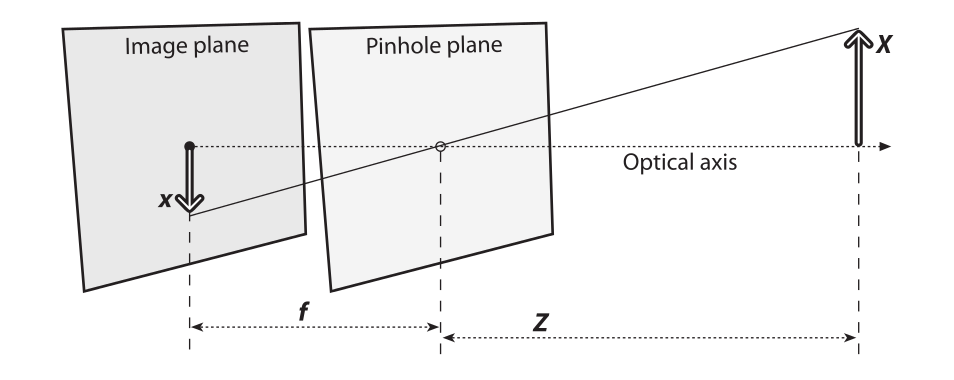
\includegraphics[scale=0.4]{./images/calib1.png} 
\caption{Rappresenzazione di un pinhole camera model} 
\label{fig:calib1}
\end{figure} 

In tale figura \em{f} è la \em{focal lenght} della telecamera, \textit{Z} la distanza tra oggetto e telecamera, \em{X} la dimensione dell'oggetto e \em{x} l'immagine dell'oggetto proiettata sul piano. \\ Il modello appena descritto può essere reinterpretato come in figura ~\ref{fig:calib2} 
\begin{figure}[htpb] 
\centering 
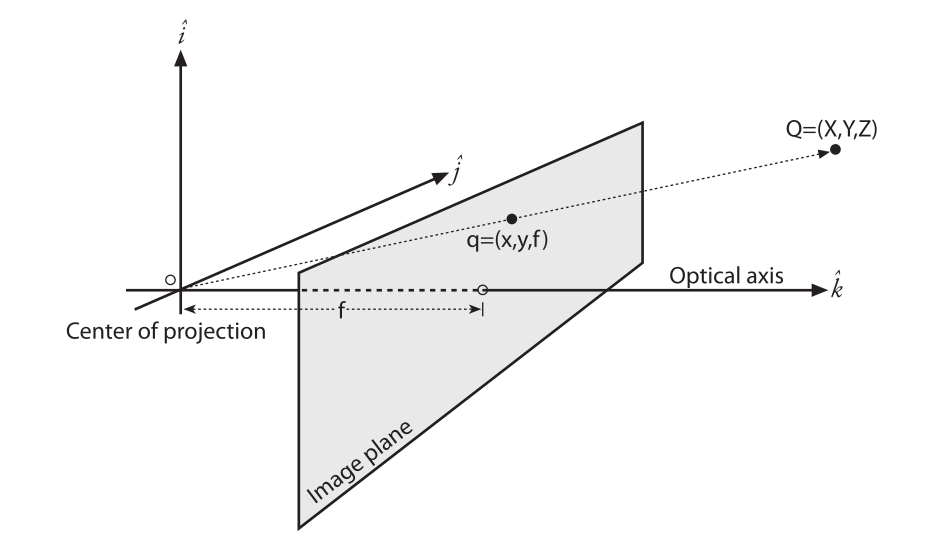
\includegraphics[scale=0.4]{./images/calib2.png} 
\caption{Rappresenzazione di un pinhole camera model rovesciato} 
\label{fig:calib2}
\end{figure} 

nella quale sono stati rovesciati il punto di \textit{pinhole} e l'\textit{image plane}. Ciò ci permette di semplificare le relazioni che valgono tra i punti dell'oggetto e le loro proiezioni. Infatti ora è più chiara la similarità dei triangoli, inoltre l'immagine non è più capovolta come era in figura ~\ref{fig:calib1}. In tale visione vanno aggiunti altri due nuovi parametri \em{c\textsubscript{x} }e \em{c\textsubscript{y}} per considerare un eventuale \textit{displacement} del centro delle coordinate sull'\textit{image plane}, dovuto alla possibilità che il centro del chip (della telecamera) non risieda esattamente sopra l'asse indicato in figura ~\ref{fig:calib2} come \textit{optical axis}. \\ \\
In tale visualizzazione c'è una semplice relazione che mappa i punti \em{Q\textsubscript{i}} nello spazio (coordinate (\em{X\textsubscript{i}},\em{Y\textsubscript{i}},\em{Z\textsubscript{i}})) nei punti sul piano di proiezione (coordinate (\em{x\textsubscript{i}},\em{y\textsubscript{i}})), tale relazione è chiamata \textit{projective transform}. Viene riportata in figura ~\ref{fig:calib3}
\begin{figure}[htpb] 
\centering 
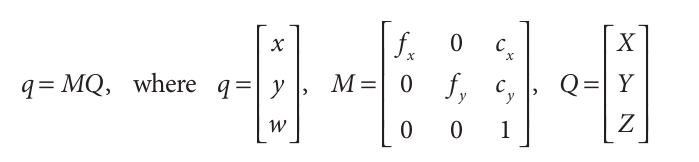
\includegraphics[scale=0.4]{./images/calib3.png} 
\caption{Espressione matematica di una relazione projective transform} 
\label{fig:calib3}
\end{figure} 

Tale modello è utile per capire la meccanica della geometria tridimensionale di visione, ma non è utilizzato nella realtà perche presenta dei limiti. Esso infatti in pratica porterebbe a una frequenza di generazione dei frame molto lenta, dovuta alla bassa quantità di luce che riesce a passare attraverso un \textit{pinhole}. Per ottenere una maggiore quantità di luce e quindi un maggior rapporto di frame/secondo è necessario utilizzare una lente, che consente di raccogliere molta più luce e di curvarla in maniera che converga nel punto di projection. Lo svantaggio di utilizzare una lente è che viene introdotta la \textit{distortion}. \\ \\

\subsubsection{Distortion parameters}

La \textit{lens distortion} si può dividere in due principali tipi:
\begin{enumerate}
	\item \textit{radial distortion}
	\item \textit{tangential distortion}
\end{enumerate}

La prima è un risultato della forma fisica della lente. Le lenti infatti tendono a distorcere i pixel vicini ai bordi dei frame, tale fenomeno è chiamato "barrel effect". Viene riportata in figura ~\ref{fig:calib4} uno schema che aiuta l'intuizione del motivo per cui tale fenomeno si verifica.
\begin{figure}[htpb] 
\centering 
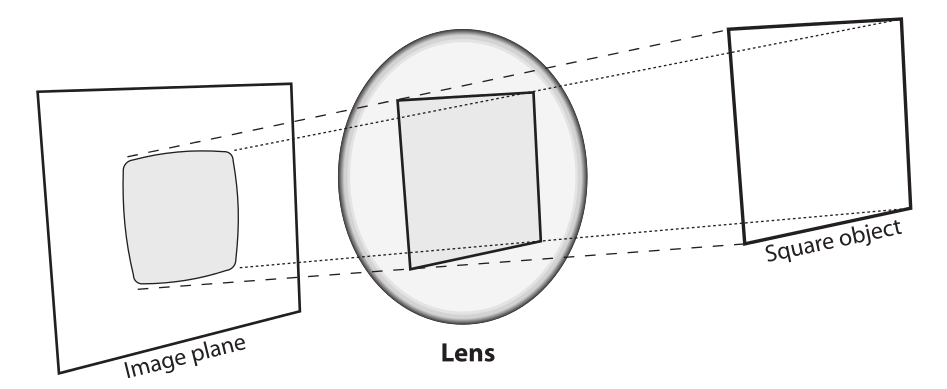
\includegraphics[scale=0.3]{./images/calib4.png} 
\caption{Radial distortion effect} 
\label{fig:calib4}
\end{figure} 
\\ \\
La seconda è un risultato dei difetti di assemblaggio che portano la lente a non essere perfettamente parallela all'\textit{image plane}. Si riporta un immagine che evidenzia tale fenomeno in figura ~\ref{fig:calib5}.
\begin{figure}[htpb] 
\centering 
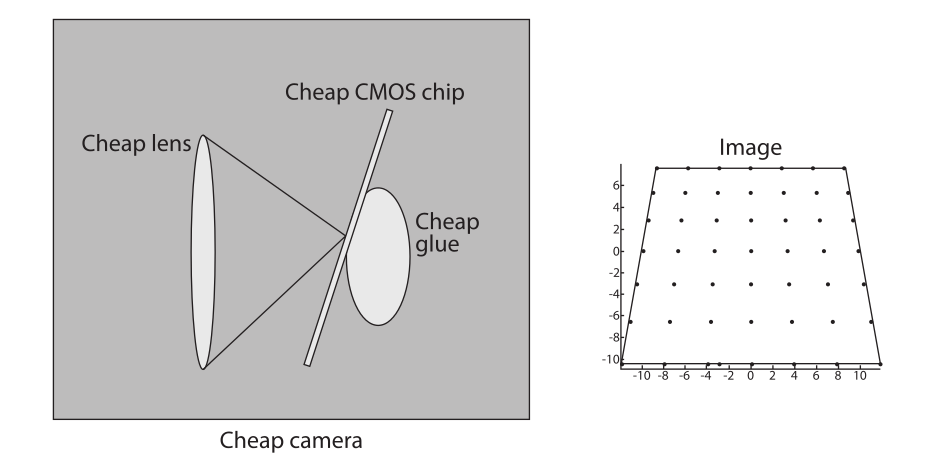
\includegraphics[scale=0.3]{./images/calib5.png} 
\caption{Tangential distortion effect} 
\label{fig:calib5}
\end{figure} 

\subsubsection{Calibrazione}

Ora che è stato descritto come identificare a livello matematico le proprietà \textit{intrinsics} e \textit{distortion} possiamo vedere le tecniche con le quali si prendono in considerazione tali parametri per correggere i frame catturati dalla telecamera.\\
Le tecniche di calibrazione si basano sul seguente criterio: viene esposto mostrato alla camera un oggetto di cui si conosce la struttura, e si valutano le differenze tra le caratteristiche dell'oggetto catturato dalla camera (quindi proiettato sull'\textit{image plane}) con le sue note caratteristiche fisiche. \\Per ogni immagine che una telecamera cattura di un oggetto, è possibile descrivere la sua posizione rispetto al sistema di coordinate della telecamera in termini di rotazione e traslazione. Possiamo quindi definire una relazione tra la posizione nello spazio di un oggetto e le sue coordinate nel frame catturato dalla telecamera. Combinando tale relazione con le correzioni derivanti dai parametri di \textit{intrinsics} si ottiene un sistema di equazioni che risolto rappresenta la soluzione al problema della calibrazione.\\
In linea di principio qualsiasi oggetto può essere usato ai fini di tale operazione, ma è pratico utilizzare un oggetto che presenta caratteristiche regolari (pattern). All'interno del progetto verrà utilizzata una immagine di una scacchiera con dimensioni (numero di celle) predefinite.  \\
Si potrà vedere come OpenCV offre un API di alto livello per la soluzione del problema della calibrazione con l'utilizzo di una scacchiera.

\subsection{Tracking data transformation}

Il sistema di \textit{video analytics} utilizza le funzionalità offerte da OpenCV per tracciare i movimenti delle persone. Non scenderemo nei dettagli di come ciò viene effettivamente implementato, basti sapere che il sistema è in grado di tracciare diversi oggetti contemporaneamente. Si riporta uno screenshot che mostra il risultato di tale operazione in ~\ref{fig:track1}.
\begin{figure}[htpb] 
\centering 
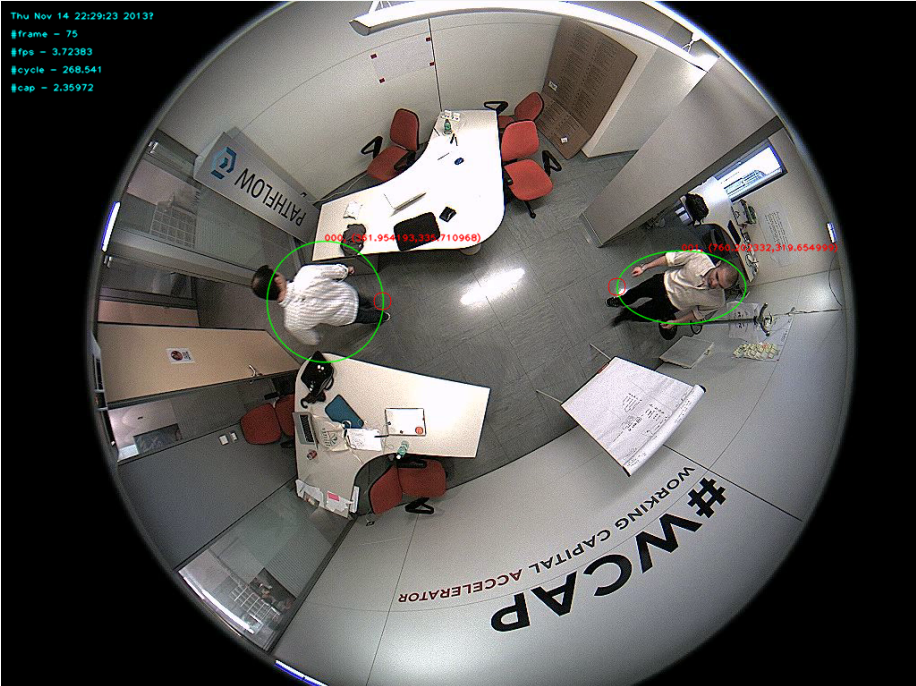
\includegraphics[scale=0.4]{./images/track1.png} 
\caption{Screenshot preso dallo stream video della camera che mostra come gli oggetti vengono tracciati} 
\label{fig:track1}
\end{figure} 
 L'output di tale processo consiste di un timestamp e delle coordinate (\textit{x} e \textit{y}) che esprimono la posizione dell'oggetto all'interno del frame della telecamera. Il sistema di coordinate che OpenCV utilizza per esprimere tali posizioni considera la posizione dell'origine in basso a sinistra del frame, ed ovviamente si basa su interi in quanto considera come unità sugli assi il pixel (ogni pixel nel frame indica una posizione).
Tali dati contengono le informazioni di tracciamento ma non sono direttamente utilizzabili in quanto il tipo di elaborazione che il progetto si propone di fare si basa su delle coordinate che non sono relative ad un particolare frame ma che sono relative ad una piantina (planimetria) del locale dove sono presenti le telecamere. Per questo è necessario che tali dati (che chiameremo \textit{raw}) vengano trattati per essere trasformati in dati che contengono l'informazione pulita e utilizzabile. Per ottenere tutto ciò è necessario avvalersi di una matrice di trasformazione (\textit{homography matrix}).
\subsubsection{Homography matrix}

Nella \textit{computer vision} viene definita come \textit{planar homography} una relazione che esprime una mappatura da un piano ad un altro. Tale relazione può essere espressa da una matrice (solitamente indicata con \textit{H}), la quale applicata ad un vettore che esprime una posizione nel piano di partenza dà come risultato una posizione nel piano di arrivo. Per calcolare tale matrice è sufficiente avere 4 punti sul piano di partenza e le loro corrispettive coordinate sul piano di arrivo. In figura ~\ref{fig:track2} si riporta una rappresentazione grafica di tale situazione.
\begin{figure}[htpb] 
\centering 
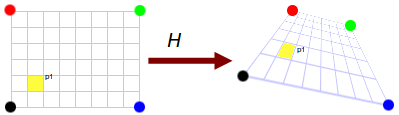
\includegraphics[scale=1.0]{./images/track2.png} 
\caption{I 4 punti necessari per il calcolo della homography matrix} 
\label{fig:track2}
\end{figure} 

Una volta che si hanno a disposizione i punti sui due piani ci sono degli algoritmi noti per calcolare la soluzione del sistema (la matrice). Una volta ottenuta la \textit{homography matrix} è facile anche effettuare l'operazione inversa: la conversione di un punto sul piano di arrivo nel suo corrispettivo nel piano di partenza.  \\ \\
All'interno del progetto verrà definito come piano di partenza il "pavimento" del locale dal punto di vista della telecamera, e come piano di arrivo la planimetria del locale. Una volta calcolata la relazione tra i due piani essa verrà utilizzata per trasformare i dati \textit{raw} che escono in output dal processo di tracking in dati puliti (relativi alla planimetria del locale).
Vedremo che OpenCV offre delle funzioni di alto livello per effettuare tale operazione.

\subsection{Qt drawings}
Qt offre molte facilitazioni per eseguire manipolazioni grafiche. All'interno del progetto è stato necessario prima di tutto convertire un immagine contenuta in un file .DXF in un immagine .PNG. Per fare ciò si sono importate alcuni degli elementi presenti nell'immagine vettoriale (i più importanti) e si sono convertiti in elementi \textbf{disegnabili} (per i quali era presente una funzione che permettesse la loro fedele rappresentazione) dalle classi di Qt. Per fare ciò lo stagista ha dovuto tenere conto delle differenze tra il sistema di coordinate utilizzato in un file .DXF e la loro rappresentazione in un sistema Qt-style. Infatti all'interno delle librerie Qt (in particolare ci riferiamo alla classe QPainter che è stata effettivamente utilizzata per disegnare) il sistema di coordinate non è standard (con origine in basso a sinistra) ma è rovesciato specularmente rispetto all'asse x. Ciò ha comportato un ulteriore passaggio. Si riporta in figura ~\ref {fig:qtgrad1} un'immagine chiarificatrice di tale situazione.


\begin{figure}[htpb] 
\centering 
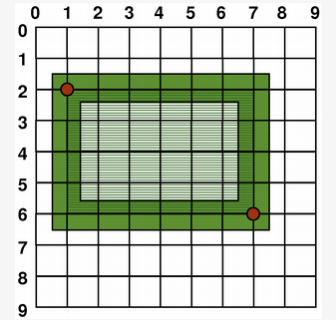
\includegraphics[scale=0.5]{./images/qtgrad1.png} 
\caption{Sistema di coordinate utilizzato per il disegno su Qt} 
\label{fig:qtgrad1}
\end{figure} 

Tale complicazione è sorta anche nell'interpretazione dei dati in output dal sistema di \textit{video analytics} utilizzati per il disegno dell'\textit{heatmap}. Tali dati (come per gli elementi nel file .DXF) utilizzano un sistema di coordinate standard (origine in basso a sinistra). E' quindi stato necessario tenere conto di tale diversità per produrre un risultato coerente.  \\ \\
Per il disegno dell'\textit{heatmap} è stato necessario l'utilizzo di \textbf{gradienti di colore}. Nella computer graphics un gradiente è una struttura che definisce una regione la cui colorazione dipende dalla posizione relativa alla "zona" coperta dal gradiente. 
Per il disegno di una mappa di calore i gradienti utilizzati sono di tipo \textit{radial}: essi sono definiti come delle zone circolari che hanno un determinato colore nel loro centro e un diverso colore ai bordi. Il colore effettivo dei punti interni è calcolato in base alla distanza dal centro del cerchio. \\
Fortunatamente Qt mette a disposizione la classe QGradient (e  derivate) che implementano il \textit{fillings} di particolari zone con gradienti.


\newpage

%%%%%%%%%%%%%%%%%%%PROGETTAZIONE DEL SISTEMA%%%%%%%%%%
\section{Progettazione} \label{sec:progett}

\subsection{Architettura Generale} \label{sec:archgen}
Le specifiche del sistema concordate con l'azienda richiedevano esplicitamente che il sistema fosse realizzato seguendo lo stile architetturale \textit{three tier} (come esplicitato nei requisiti).  \\
Dato tale vincolo si è progettato il sistema affinché esso fosse rispettato, per fare ciò si sono definiti i tre livelli del pattern (\textit{user interface, business layer, data access layer}) come i tre package di alto livello. Il package UserInterface si occuperà della presentazione dei dati e dell'interfaccia utente, il package BusinessLayer conterrà la logica dell'applicazione, il package DataAccessLayer si occuperà di fornire l'accesso ai dati dell'applicazione (contenuti in un database). Si sono ulteriormente separate le funzionalità di ciascun livello in sotto-componenti i quali raggruppano insiemi di funzionalità affini. \\
Si allega il diagramma dei package che descrive l'architettura generale dell'applicazione in figura ~\ref{fig:archgen}.\\\\

\begin{figure}[htpb]
\centering
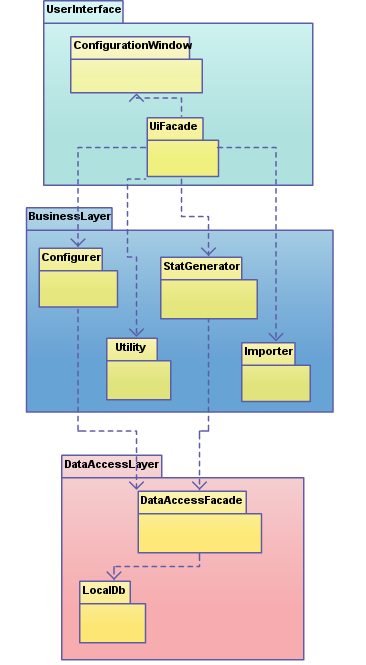
\includegraphics[scale=0.5]{./images/archgen.png}
\caption{Diagramma dei package del sistema}
\label{fig:archgen}
\end{figure}
La motivazione di tale scelta nasce dalla necessità di voler massimizzare l'indipendenza di ogni livello rispetto al resto del sistema. Sia per quanto riguarda il livello dei dati che quello di presentazione infatti era richiesto che fossero sostituibili in blocco senza andare a modificare le altre componenti dell'applicazione. Si è preferita tale decisione per far fronte (in particolare) ad eventuali necessità di sostituzione di librerie grafiche (Qt) oppure di tipo di database, infatti il team di sviluppo non è stato in grado di garantire che MySql sarebbe riuscito a tenere dei tempi di risposta soddisfacenti all'aumentare della complessità e della cardinalità dei dati.


\subsection{Utilizzo MVC} \label{sec:mvc}
Nelle prime fasi di analisi quando è stato esplicitato che il sistema avrebbe dovuto essere strutturato secondo un'architettura in stile \textit{three-tier}, si è svolta una riunione nella quale lo stagista ha proposto di utilizzare invece il pattern MVC. \\
L'MVC infatti avrebbe garantito uno sviluppo leggermente più veloce, in quanto le componenti sono maggiormente legate (rispetto ad un architettura a layers) e quindi non c'è la necessità di separare completamente le strutture e i tipi utilizzati in ognuna di esse. Inoltre dal punto di vista dello stagista l'MVC si prestava meglio al tipo di programma che andava prodotto, infatti esso avrebbe dovuto funzionare  in ambito Desktop e avrebbe richiesto interazione diretta da parte di un'utente addetto alla configurazione. \\ \\
Il team di sviluppo ha quindi esplicitato alcuni obiettivi che il software avrebbe in futuro dovuto raggiungere. E' stato chiarito che le componenti dovessero essere quanto più separate e indipendenti tra loro possibile perché l'obiettivo futuro era quello di rendere disponibile l'interazione con l'applicazione da remoto. L'idea di fondo infatti è che quando il sistema avrà raggiunto un sufficiente grado di stabilità tutta la parte di amministrazione (e configurazione) verrà portata fuori dallo store locale e messa online. \\
Le motivazioni di questa scelta sono soprattutto legate alle difficoltà logistiche che la configurazione in locale avrebbe comportato qualora le installazioni avessero raggiunto una distribuzione molto ampia e sparsa (eventualmente anche a livello internazionale). \\ 
Per questo motivo era preferibile mantenere una struttura a layers, che potesse massimizzare non solo l'indipendenza tra le diverse funzionalità, ma anche quella tra layer, in maniera che in futuro sarebbe stato più semplice legare l'esecuzione di un comando ad una singola chiamata di metodo. \\ \\
D'altro canto non si è puntato subito a tale obiettivo (accesso e configurazione da remoto) in quanto si è ritenuto preferibile partire con un primo prototipo (che sarebbe entrato in \textit{beta testing} su 2 negozi Telecom di Roma) che fornisse un'interfaccia semplice, ma che offrisse soprattutto la possibilità di eseguire \textit{debug}. Infatti essendo il sistema nel suo insieme molto complesso si è ritenuto necessario avere la possibilità di fare \textit{debug} sul sistema fino a che questo non avesse raggiunto una stabilità e affidabilità sufficiente per garantirne il funzionamento.


\subsection{Database schema} \label{sec:dbschema}
Si riporta di seguito uno schema del database utilizzato all'interno dell'applicazione per il salvataggio dei dati. \\
Sebbene alcuni dati fossero comunque legati ad una telecamera, si è scelto di separare le informazioni in tabelle diverse per coerenza e semplicità. Si sono quindi divise le informazioni riguardanti la calibrazione nella tabella \textbf{tbl_cam_calibration} e nella tabella \textbf{tbl_cam}.\\
Si riporta una breve spiegazione che motiva le scelte effettuate nella progettazione dello schema del database:
\begin{enumerate}
	\item Tra \textbf{tbl_cam} e \textbf{tbl_homographic_matrices} c'è una relazione di tipo 1:N. Si è optato per tale decisione per permettere in futuro di associare diverse \textit{homography matrix} alla stessa telecamera, ciò consente al sistema di salvare matrici diverse che esprimono relazioni diverse tra le coordinate dei punti tracciati e la loro reale rappresentazione sulla planimetria del locale. In tale modo senza perdere di consistenza si possono effettuare \textit{zoom} e rotazioni per ottenere maggiori dettagli dai dati
	\item Il campo \textbf{transformed} nella tabella \textbf{tbl_tracking_data} serve per memorizzare la condizione del dato. Infatti dato che i processi di salvataggio e successiva trasformazione non sono collegati tra di loro ma comunicano con la stessa base dati, è importante sapere se un dato è già stato "trasformato" e quindi spostato nella tabella \textbf{tbl_clean_data} oppure se tale operazione ancora non è stata eseguita. Tale campo memorizza un booleano che indica lo stato del record
	\item La tabella \textbf{tbl_clean_data} memorizza i dati di tracciamento relativi al locale nel suo complesso (la planimetria). Essa contiene i dati di tracciamento ottenuti dopo la loro trasformazione del loro valore \textit{raw} in dati \textit{clean}: essi sono relativi all'intera area del locale e non più legati ad una telecamera (infatti ogni telecamera ha delle regole di trasformazione del dato da essa catturato personalizzate, che dipendono dalla matrice omografica usata per la traduzione). In tale modo anche con un sistema funzionante con diverse telecamere si crea un dato unificato e pulito utilizzabile per la generazione delle statistiche. Similmente al campo transformed di cui sopra, il campo \textbf{synchronized} indica se il dato è già stato salvato in un sistema di backup (distribuito)
\end{enumerate}
Lo schema del database è allegato in figura ~\ref{fig:dbschema}.

\begin{figure}[!h]
\centering
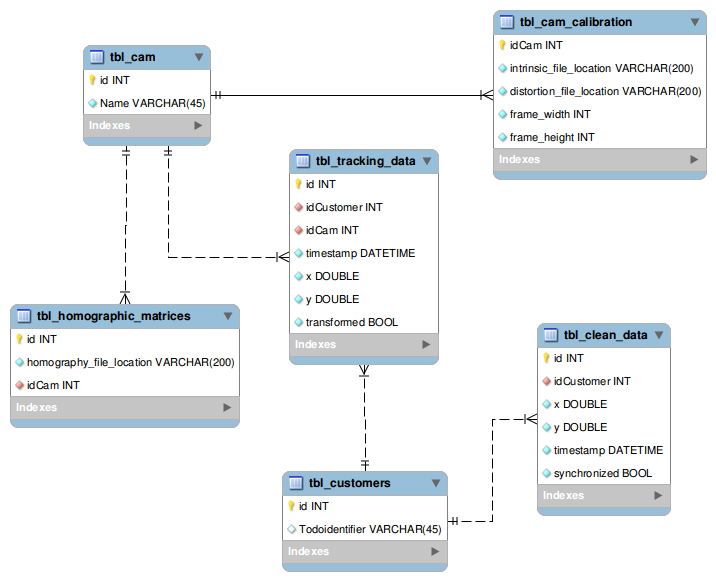
\includegraphics[scale=0.5]{./images/dbschema.png}
\caption{Schema del database locale (MySql Workbench editor)}
\label{fig:dbschema}
\end{figure}

\newpage
\subsection{Specifica} \label{sec:specifica}
\subsubsection{C1 - UserInterface} \label{sec:c1}
Componente che rappresenta il livello \textit{user interface} nell'architettura three tier dell'applicazione. Esso contiene l'interfaccia grafica visibile all'utente, ed è responsabile della presentazione dei dati e della corretta interpretazione degli eventi utente e del loro inoltro nei livelli inferiori. Contiene le finestre del programma, cioè finestra principale, finestra di configurazione, finestra di calibrazione. \\
\begin{figure}[!h] 

        \centering 

        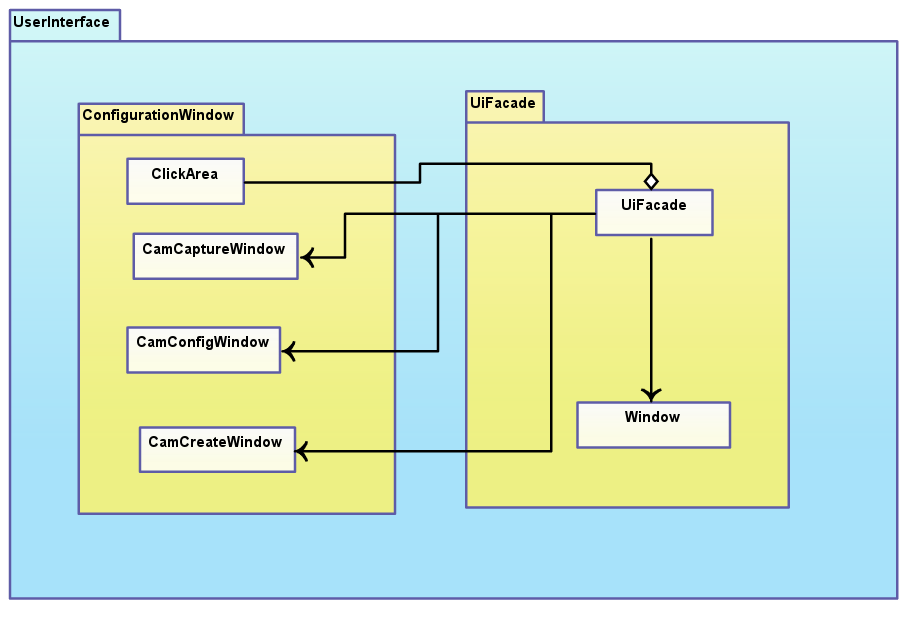
\includegraphics[scale=0.4]{./images/c1.png} 

        \caption{C1 - UserInterface} 

        \label{fig:c1}

        \end{figure} 

Relazioni con altri componenti: 
\begin{itemize} 
\item [\textbf{C2}]
Il livello di presentazione (UI) utilizza il livello logico per inoltrare e quindi rispondere agli eventi utente. Ogni richiesta infatti viene delegata al livello sottostante il quale è responsabile per la risoluzione e la risposta ad essa 
\end{itemize} 

\subsubsection{C1.1 - UserInterface::ConfigurationWindow} \label{sec:c1.1}
Tale componente si occupa della presentazione delle finestre di configurazione del sistema. \\
Classi contenute nel componente: 
\begin{itemize} 
\item \textbf{ClickArea}
\begin{description}
\item [\textit{descrizione e utilizzo:}] Rappresenta un'area dove le coordinate dei click dell'utente vengono trattate in una particolare maniera e memorizzate in dei campi per una successiva elaborazione. Viene utilizzata per il calcolo della matrice omografica che permette la mappatura dei dati di tracking, memorizza i punti cliccati dall'utente affinché possano in seguito essere recuperati e passati alle classi che li elaborano
\item [\textit{classi ereditate:}] QLabel
\end{description}
\item \textbf{CamCaptureWindow}
\begin{description}
\item [\textit{descrizione e utilizzo:}] Rappresenta la finestra che aiuta l'utente a salvare (direttamente dallo stream della telecamera) o inserire (dal file system) un frame della telecamera. Viene utilizzata per svolgere tale funzione, offre sia la possibilità di catturare un'immagine dal video stream sia quella di selezionare un file dal disco da utilizzare per il calcolo della \textit{homography matrix}
\item [\textit{classi ereditate:}] QWidget
\end{description}
\item \textbf{CamCreateWindow}
\begin{description}
\item [\textit{descrizione e utilizzo:}] Rappresenta la finestra per l'inserimento di una nuova telecamera. Essa viene utilizzata per l'inserimento di una nuova configurazione relativa ad una telecamera nel sistema. Fornisce all'utente il campo dove inserire il nome della telecamera e segnala l'azione di inserimento 
\item [\textit{classi ereditate:}] QWidget
\end{description}
\item \textbf{CamConfigWindow}
\begin{description}
\item [\textit{descrizione e utilizzo:}] Rappresenta la finestra che permette all'utente di gestire la configurazione delle telecamere. Viene utilizzata per tutte le modifiche di tali informazioni (insert, update, delete) su ogni dato salvato nel database, cioè informazioni di calibrazione, matrice omografica associata, e nome della telecamera
\item [\textit{classi ereditate:}] QWidget
\end{description}
\end{itemize}

\subsubsection{C1.2 - UserInterface::UiFacade} \label{sec:c1.2}
Componente che si occupa della visualizzazione della finestra principale del programma e del corretto inoltro delle richieste e degli eventi provenienti dal livello di \textit{user interface} ai livelli inferiori.\\
Relazioni con altri componenti: 
\begin{itemize} 
\item [\textbf{C1.1}]
Il componente tiene il controllo di tutte le finestre del sistema, quindi utilizza ConfigurationWindow ~\ref{sec:c1.1} per accedere alle finestre di configurazione. E' responsabile per la loro corretta visualizzazione e l'interpretazione dei loro segnali 
\item [\textbf{C2.1}]
Il componente utilizza le funzionalità messe a disposizione da Configurer ~\ref{sec:c2.1} per rispondere alle richieste di configurazione dell'utente 
\item [\textbf{C2.2}]
Il componente utilizza le funzionalità messe a disposizione da Importer ~\ref{sec:c2.2} per rispondere alle richieste riguardanti l'importazione dei file .DXF e la loro conversione e visualizzazione. 
\item [\textbf{C2.3}]
Il componente utilizza le funzionalità messe a disposizione da StatGenerator ~\ref{sec:c2.3} per rispondere alle richieste di visualizzazione statistiche o generazione delle stesse 
\item [\textbf{C2.4}]
Il componente utilizza le funzionalità messe a disposizione da Utility ~\ref{sec:c2.4} per svolgere le funzioni di utilità 
\end{itemize} 

Classi contenute nel componente: 
\begin{itemize} 
\item \textbf{UiFacade}
\begin{description}
\item [\textit{descrizione e utilizzo:}] Rappresenta il facade utilizzato per convogliare in un unico punto tutte le richieste uscenti dal livello di presentazione verso i livelli sottostanti. Essa viene utilizzata per tale scopo, infatti tutte le altre classi di interfaccia segnalano gli eventi utente a UiFacade che si occupa di inoltrare una precisa richiesta ai livelli sottostanti
\item [\textit{classi ereditate:}] QWidget
\end{description}
\item \textbf{Window}
\begin{description}
\item [\textit{descrizione e utilizzo:}] Finestra principale del programma. Contiene i bottoni per l'accesso alle varie funzionalità. Viene caricata all'avvio del sistema e rimane aperta per l'intera durata dell'esecuzione, gestisce gli eventi utente inoltrando i segnali verso i livelli inferiori
\item [\textit{classi ereditate:}] QWidget
\end{description}
\end{itemize}

\subsubsection{C2 - BusinessLayer} \label{sec:c2}
Componente che rappresenta il livello \textit{business layer} nell'architettura three tier dell'applicazione. Esso contiene le classi che contengono la logica dell'applicazione, ed è responsabile della corretta risoluzione delle chiamate provenienti dall'\textit{user interface}. Esso è inoltre incaricato di gestire gli errori e di segnalarli.
\\
\begin{figure}[!h] 

        \centering 

        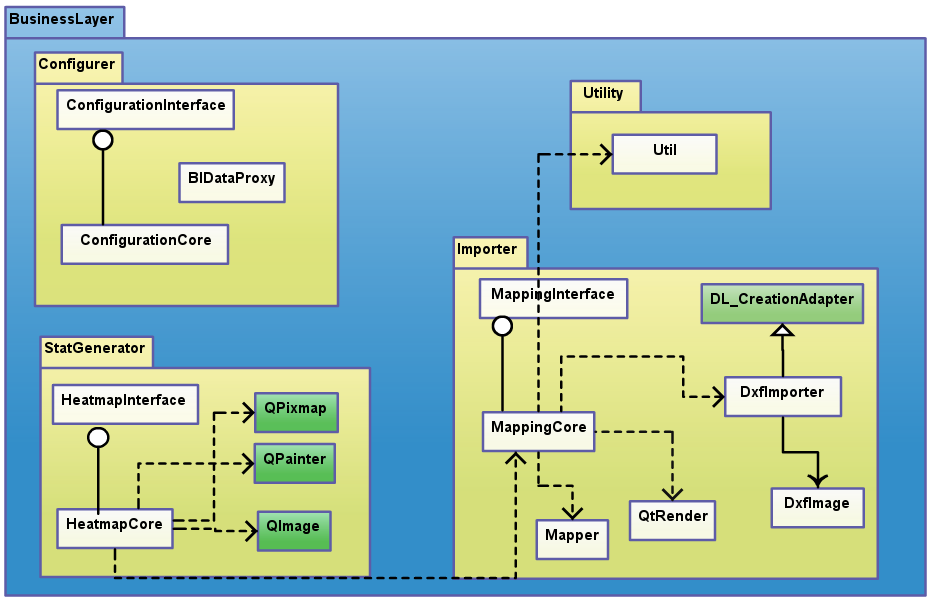
\includegraphics[scale=0.4]{./images/c2.png} 

        \caption{C2 - BusinessLayer} 

        \label{fig:c2}

        \end{figure} 

Relazioni con altri componenti: 
\begin{itemize} 
\item [\textbf{C3}]
Il livello logico (BL) utilizza il livello di \textit{data access} ogni volta che ha necessità di reperire informazioni memorizzate in un database o di modificarle (select, insert, update, delete). Una volta che ha ottenuto il dato o eseguito l'operazione la interpreta e agisce di conseguenza (stato di errore, corretta terminazione) 
\end{itemize} 

\subsubsection{C2.1 - BusinessLayer::Configurer} \label{sec:c2.1}
Componente che è responsabile per le funzionalità di configurazione del sistema.\\
Relazioni con altri componenti: 
\begin{itemize} 
\item [\textbf{C3.1}]
Utilizza DataAccessFacade ~\ref{sec:c3.1} per accedere ai dati dell'applicazione. Vi delega le operazioni sul database 
\end{itemize} 

Classi contenute nel componente: 
\begin{itemize} 
\item \textbf{ConfigurationInterface}
\begin{description}
\item [\textit{descrizione e utilizzo:}] Classe astratta che definisce l'interfaccia per la configurazione delle telecamere del sistema. Viene implementata e i suoi metodi vengono ridefiniti per fornire le funzionalità di configurazione richieste
\end{description}
\item \textbf{ConfigurationCore}
\begin{description}
\item [\textit{descrizione e utilizzo:}] Ridefinisce e ConfigurationInterface. Implementa metodi necessari per la configurazione delle telecamere nel sistema. Fornisce i metodi per eseguire inserimento, modifica e cancellazione delle informazioni presenti nelle tabelle del database locale
\item [\textit{classi ereditate:}] ConfigurationInterface
\end{description}
\item \textbf{BlDataProxy}
\begin{description}
\item [\textit{descrizione e utilizzo:}] Fornisce un accesso unificato per il solo recupero (select) dei dati salvati nel sistema. Raggruppa tutti i metodi di selezione necessari al livello di interfaccia per presentare i dati. Viene utilizzata da UiFacade come ponte per l'accesso ai dati presenti nel database
\end{description}
\end{itemize}

\subsubsection{C2.2 - BusinessLayer::Importer} \label{sec:c2.2}
Componente responsabile per le funzionalità di importazione dei file .DXF e la loro conversione e rendering in immagine. \\
Classi contenute nel componente: 
\begin{itemize} 
\item \textbf{MappingInterface}
\begin{description}
\item [\textit{descrizione e utilizzo:}] Classe astratta che definisce l'interfaccia per le funzionalità di \textit{mapping}. Viene implementata e i suoi metodi vengono ridefiniti per fornire le funzionalità di importazione e generazione della \textit{homography matrix}
\end{description}
\item \textbf{MappingCore}
\begin{description}
\item [\textit{descrizione e utilizzo:}] Ridefinisce MappingInterface. Implementa i metodi necessari per l'importazione e il \textit{mapping} dei dati per renderli direttamente utilizzabili per il calcolo di statistiche. Utilizza i metodi contenuti nelle altre classi del componente (quali \textbf{Mapper}, \textbf{QtRender}, \textbf{DxfImporter})
\item [\textit{classi ereditate:}] MappingInterface
\end{description}
\item \textbf{DxfImage}
\begin{description}
\item [\textit{descrizione e utilizzo:}] Descrive un immagine contenuta in un file di tipo .DXF. Contiene dei riferimenti a delle strutture che rappresentano gli elementi (quelli che vengono importati) contenuti nel file. Viene utilizzata per l'importazione dei file .DXF oltre che per la loro successiva rappresentazione grafica

\end{description}
\item \textbf{DxfImporter}
\begin{description}
\item [\textit{descrizione e utilizzo:}] Eredita la classe astratta fornita dalla libreria dxflib definita per il \textit{parsing} e l'importazione dei file .DXF. Converte le strutture fornite dalla classe nelle strutture proprie del sistema, poi le aggiunge ad un oggetto di tipo DxfImage per la memorizzazione. Viene utilizzata nell'importazione e nel parsing dei file .DXF
\item [\textit{classi ereditate:}] DL_CreationAdapter
\end{description}
\item \textbf{QtRender}
\begin{description}
\item [\textit{descrizione e utilizzo:}] Classe che si occupa di fare il \textit{render} di un'immagine contenuta in una classe di tipo DxfImage su un oggetto di tipo QPixmap (che rappresenta un immagine bitmap sulla quale poter disegnare). Utilizza la classe QPainter per disegnare, e viene utilizzata per la visualizzazione dei file .DXF importati e la loro conversione in formato .PNG
\end{description}
\item \textbf{Mapper}
\begin{description}
\item [\textit{descrizione e utilizzo:}] Classe che raggruppa le funzionalità di \textit{mapping}. Essa viene utilizzata dalle classi che si occupano di della mappatura per l'esecuzione dei metodi basilari che  sono: calcolo della matrice omografica e applicazione della trasformazione ad un punto
\end{description}
\end{itemize}

\subsubsection{C2.3 - BusinessLayer::StatGenerator} \label{sec:c2.3}
Componente responsabile per la generazione delle statistiche di tracking a partire dai dati del sistema. \\
Relazioni con altri componenti: 
\begin{itemize} 
\item [\textbf{C3.1}]
Utilizza DataAccessFacade ~\ref{sec:c3.1} per accedere ai dati dell'applicazione. Recupera le informazioni sui dati per la generazione delle statistiche richieste 
\end{itemize} 

Classi contenute nel componente: 
\begin{itemize} 
\item \textbf{HeatMapInterface}
\begin{description}
\item [\textit{descrizione e utilizzo:}] Classe astratta che definisce l'interfaccia per le funzionalità di generazione \textit{heatmap}. Viene implementata e i suoi metodi vengono ridefiniti per fornire il metodo di generazione heatmap
\end{description}
\item \textbf{HeatmapCore}
\begin{description}
\item [\textit{descrizione e utilizzo:}] Ridefinisce HeatMapInterface. Implementa i metodi necessari per la generazione dell'\textit{heatmap}. Utilizza un gradiente salvato nella directory di esecuzione del programma per scegliere le gradazioni del colore nella mappa, segnala l'errore se tale file è mancante
\item [\textit{classi ereditate:}] HeatMapInterface
\end{description}
\end{itemize}

\subsubsection{C2.4 - BusinessLayer::Utility} \label{sec:c2.4}
Componente che contiene alcune funzionalità di utility. Esse vengono messe a disposizione per i livelli superiori del sistema.\\
Classi contenute nel componente: 
\begin{itemize} 
\item \textbf{Util}
\begin{description}
\item [\textit{descrizione e utilizzo:}] Classe contenitore per le funzioni di utilità del sistema. Fornisce un raggruppamento per i metodi che eseguono operazioni comuni a tutto il programma. Viene utilizzata sia dal livello superiore che da altre classi del BusinessLayer per eseguire alcune funzionalità che sono comuni
\end{description}
\end{itemize}

\subsubsection{C3 - DataAccessLayer} \label{sec:c3}
Componente che rappresenta il livello di \textit{data access layer} nell'architettura three tier dell'applicazione. Esso fornisce le funzionalità per l'accesso ai dati del sistema, che sono salvati in maniera persistente in dei database. 
\\
\begin{figure}[!h] 

        \centering 

        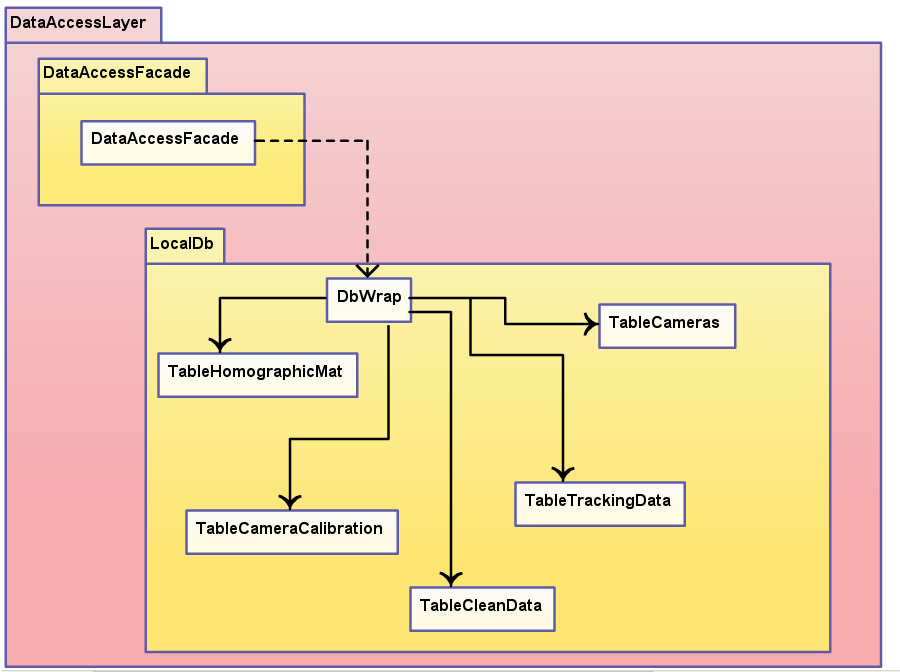
\includegraphics[scale=0.4]{./images/c3.png} 

        \caption{C3 - DataAccessLayer} 

        \label{fig:c3}

        \end{figure} 

\subsubsection{C3.1 - DataAccessLayer::DataAccessFacade} \label{sec:c3.1}
Componente che rappresenta un \textit{facade} per l'effettivo accesso alle funzionalità del \textit{data access layer}. Esso si occupa di fornire una via unificata di accesso per i possibili database differenti con cui l'applicazione si deve interfacciare\\
Relazioni con altri componenti: 
\begin{itemize} 
\item [\textbf{C3.2}]
Utilizza LocalDb ~\ref{sec:c3.2} per accedere ai metodi specifici del database locale, vi inoltra quindi le richieste di insert, update, delete, select 
\end{itemize} 

Classi contenute nel componente: 
\begin{itemize} 
\item \textbf{DataAccessFacade}
\begin{description}
\item [\textit{descrizione e utilizzo:}] La classe rappresenta un \textit{facade} per l'accesso alle funzionalità del \textit{data layer}. Essa unifica al suo interno tutte le richieste in arrivo dai livelli superiori e le indirizza alla classe appropriata. Viene utilizzata dalle classi del \textit{business layer} per l'accesso ai dati presenti nel database
\end{description}
\end{itemize}

\subsubsection{C3.2 - DataAccessLayer::LocalDb} \label{sec:c3.2}
Componente che contiene le funzionalità per l'accesso al database locale. Esso fornisce l'interfaccia per la modifica dei dati e il loro recupero\\
Classi contenute nel componente: 
\begin{itemize} 
\item \textbf{DbWrap}
\begin{description}
\item [\textit{descrizione e utilizzo:}] Classe wrapper per il database locale contentente le informazioni di configurazione delle telecamere. Essa mette a disposizione i metodi per l'accesso ai dati e la loro modifica. E' implementata come singleton per evitare allocazioni multiple. Contiene una copia statica di tutti i dati presenti nel database, per prevenire accessi ripetuti in memoria che possono causare lentezza del sistema.
\end{description}
\item \textbf{TableHomographicMat}
\begin{description}
\item [\textit{descrizione e utilizzo:}] Classe che contiene i metodi di basso livello per accedere alla tabella \textbf{tbl_homographic_matrices}
\end{description}
\item \textbf{TableTrackingData}
\begin{description}
\item [\textit{descrizione e utilizzo:}] Classe che contiene i metodi di basso livello per accedere alla tabella \textbf{tbl_tracking_data}
\end{description}
\item \textbf{TableCameras}
\begin{description}
\item [\textit{descrizione e utilizzo:}] Classe che contiene i metodi di basso livello per accedere alla tabella \textbf{tbl_cam}
\end{description}
\item \textbf{TableCameraCalibration}
\begin{description}
\item [\textit{descrizione e utilizzo:}] Classe che contiene i metodi di basso livello per accedere alla tabella \textbf{tbl_cam_calibration}
\end{description}
\item \textbf{TableCleanData}
\begin{description}
\item [\textit{descrizione e utilizzo:}] Classe che contiene i metodi di basso livello per accedere alla tabella \textbf{tbl_clean_data}
\end{description}
\end{itemize}


\subsection{Diagrammi di sequenza} \label{sec:sequenza}
Vengono riportati in questa sezione dei diagrammi di sequenza, al fine di illustrare meglio l'architettura del server.\\
Il diagramma riportato in figura~\ref{fig:seq1} mostra il flusso delle operazioni causate da un'azione dell'utente che non va a modificare i dati nel database. Si vede che l'ordine delle chiamate parte dal livello di presentazione e viene inoltrato nei livelli inferiori fino a quando viene effettivamente chiamato il metodo richiesto. Nei ritorni ci sono dei controlli che sono stati inseriti per verificare l'esito (successo/fallimento) dell'operazione in maniera che esso potesse essere segnalato. Le regole per la comunicazione tra i livelli sono uniformi e standardizzate. \\
\begin{figure}[!h]
\centering
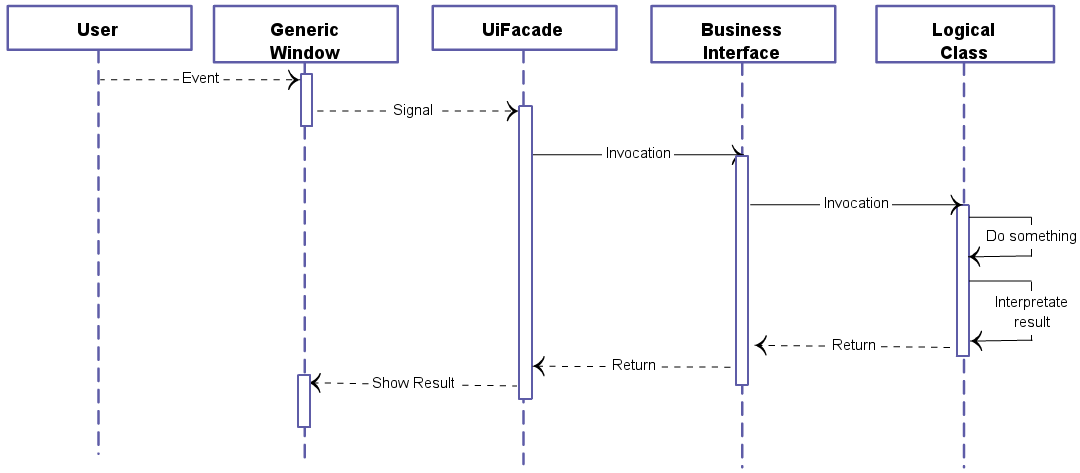
\includegraphics[scale=0.4]{./images/seq1.png}
\caption{Diagramma di sequenza, generica richiesta dell'utente}
\label{fig:seq1}
\end{figure}
Similmente il diagramma in figura~\ref{fig:seq2} riporta il flusso delle operazioni quando è coinvolto il livello dell'accesso ai dati.
\begin{figure}[!h]
\centering
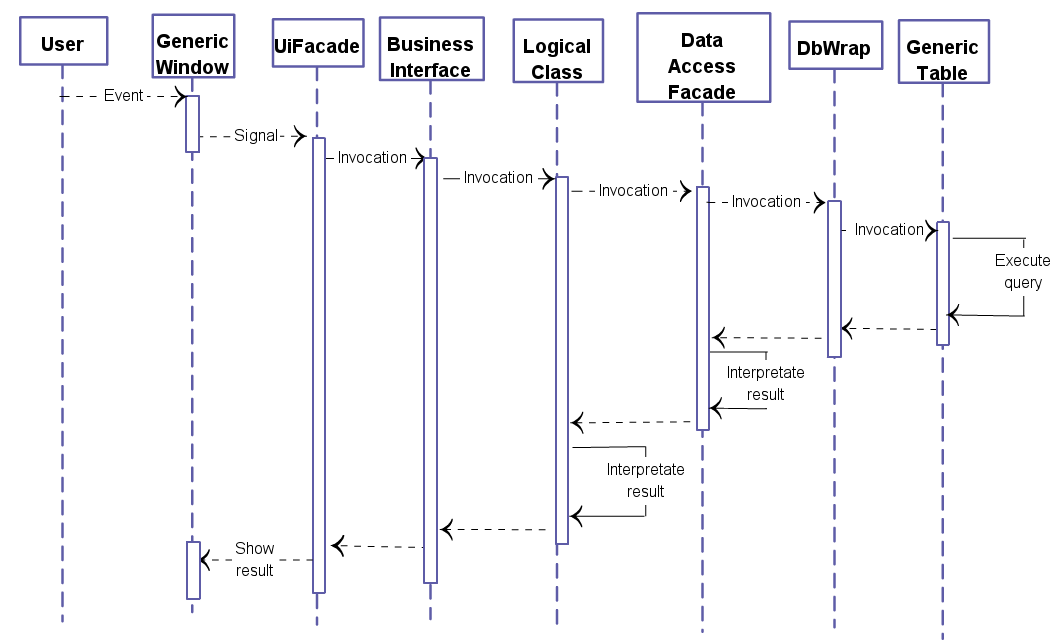
\includegraphics[scale=0.4]{./images/seq2.png}
\caption{Diagramma di sequenza, generica richiesta utentei di  modifica ai dati}
\label{fig:seq2}
\end{figure}
\clearpage
%%%%%%%%%%%%%%%%%%%%%END PROGETTAZIONE%%%%%%%%%%%%%%%%%%%

\section{Verifica e validazione} \label{sec:vev}
\subsection{Analisi statica} \label{sec:anstat}
Al fine di portare avanti il processo di verifica con metodo è stato necessario renderlo quantificabile. A tal fine si sono definite delle metriche sul codice sorgente. Esse sono di seguito definite e il loro significato viene descritto e spiegato. Per ogni metrica si sono definiti un range di accettazione e un range ottimale. \\

{\large \textbf{Complessità ciclomatica}\par} 
Tale metrica indica il numero di cammini linearmente indipendenti percorribili durante l'esecuzione di un singolo metodo. Tale metrica è molto importante in quanto ha implicazioni dirette sulle attività di testing: infatti essa rappresenta un \textit{upper bound} per il numero di routine di test necessarie per raggiungere un completo \textit{branch coverage}. \\ 
\textbf{Range definiti:}
\begin{itemize}
	\item Accettazione \textless = 20
	\item Ottimale \textless = 12
\end{itemize}

{\large \textbf{NbLinesOfCode}\par} 
Tale metrica indica il numero di righe di codice. Essa può essere considerata per i tipi, i metodi, i namespace, i progetti. Tale conteggio esclude tutte le righe di codice sorgente che non vengono eseguite. Quindi sono escluse tutte le dichiarazioni di namespaces, tipi, campi, metodi oltre che i metodi astratti e i tipi enumeration. Solo il codice effettivamente eseguito è considerato nel conteggio delle righe.\\
La metrica LOC non è sempre legata alla produttività del programmatore, ma torna utile sia nel calcolo della percentuale di statement coverage e nella valutazione del software. \\
Essa è indice di manutenibilità (è più semplice manutenere metodi brevi) e quindi qualità del codice. Nel progetto sono stati messi dei vincoli sul numero di LOC per ogni metodo per evitare che questi diventassero troppo grandi e quindi poco gestibili.
\textbf{Range definiti (per metodo):}
\begin{itemize}
	\item Accettazione \textless = 80
	\item Ottimale \textless = 20
\end{itemize}

{\large \textbf{Numero di campi per classe}\par} 
Indica il numero di membri di classe (campi dati) di una particolare classe. E' importante in quanto è indice delle responsabilità affidate ad una classe, se viene superato può indicare che la classe ne raggruppa troppe altre e andrebbe ulteriormente separata in classi distinte.
\textbf{Range definiti:}
\begin{itemize}
	\item Accettazione \textless = 16
	\item Ottimale \textless = 8
\end{itemize}

{\large \textbf{Numero di metodi per classe}\par} 
Indica il numero di metodi di una particolare classe. Similmente al numero di campi per classe è importante in quanto è indice delle responsabilità affidate ad una classe, se viene superato può indicare che la classe ha troppe funzionalità e andrebbe separata.
\textbf{Range definiti:}
\begin{itemize}
	\item Accettazione \textless = 16
	\item Ottimale \textless = 8
\end{itemize}

{\large \textbf{Numero di argomenti per metodo}\par} 
Indica il numero di argomenti passati come parametri nell'invocazione di un metodo. Metodi con troppi parametri diventano frustranti, poco manutenibili e inutilmente complessi.
\textbf{Range definiti:}
\begin{itemize}
	\item Accettazione \textless = 8
	\item Ottimale \textless = 4
\end{itemize}

{\large \textbf{Cohesion Of Methods (LCOM HS)}\par} 
Nella programmazione ad oggetti il principio detto \textit{single responsibility principle} che afferma che una classe dovrebbe incapsulare una sola responsabilità (anche detta \textit{reason to change}). Se una classe ha una sola responsabilità (rispetta il principio) si dice che essa è coesa. In generale una classe risulterà coesa se i suoi metodi sono strettamente legati fra loro. Quando metodi distinti non usano attributi o metodi comuni significa che essi non condividono nulla e che quindi potrebbero venir separati. La metrica di LCOM misura quanto poco una classe è coesa.
Alcune formule per il calcolo di LCOM sono le seguenti: \\
\begin{equation}
\begin{split}
LCOM& = 1-(\sum(a)/m*f) \\
LCOM HS& = m-(\sum(a)/f)(m-1) \\
\end{split}
\end{equation}
dove:
\begin{description}
	\item \textbf{\textit{m}} è il numero di metodi nella classe (sia statici che d'istanza)
	\item \textbf{\textit{f}} è il numero di campi dati di tipo classe all'interno della classe considerata
	\item \textbf{\textit{a}} è il numero di metodi della classe che accedono un particolare campo dati di tipo classe
\end{description}
L'idea alla base di tali formule è che una classe perfettamente coesa utilizza tutti i suoi campi dati di tipo classe all'interno di ogni suo metodo il che comporta :
\begin{equation}
\begin{split}
sum(a)& = m*f \\
LCOM& = 0\\
\end{split}
\end{equation}
La differenza tra LCOM e la sua versione HS (Hendersons-Sellers) è che la prima ritorna dei valori nel range [0-1] mentre la seconda nel range [1-2]. La versione HS è considerata più efficace per la rilevazione dei tipi scarsamente coesi. \\
Tale metrica è interessante, ma va trattata con cautela (basti pensare una classe che ha n campi dati, n \textit{getters} e n \textit{setters}, essa risulterà scarsamente coesa, il che non rispecchia la realtà). Infatti essa non va valutata singolarmente, ma deve essere inserita in un contesto di valutazione che comprende altre variabili, soprattutto il numero di campi e il numero di metodi. In generale un valore di LCOM HS \textgreater 1.0 può indicare una classe poco coesa.
\textbf{Range definiti:}
\begin{itemize}
	\item Accettazione \textless  1.0
	\item Ottimale \textgreater = 1.0
\end{itemize}

{\large \textbf{Type rank}\par}
La metrica di \textit{type rank} viene calcolata utilizzando l'algoritmo PageRank di Google sulla struttura definita dal grafo delle dipendenze tra tipi. Il \textit{type rank} medio è 1. Quello che la metrica fornisce è una valutazione di quanto una classe viene riferita dalle altre, è preferibile quindi impiegare più tempo per il testing di classi con alto rank in quanto è più facile che errori in tali classi si rivelino più pericolosi. \\
Dato che la metrica non esprime una valutazione che indica un fattore positivo o negativo, essa verrà utilizzata come indicatore per il coverage necessario per quella classe. Il criterio è il seguente: \\ se la classe ha un valore di \textit{type rank} \textgreater = 1.0 per essa verranno progettati test sufficienti per garantire un coverage \textgreater = 95 \%




\subsection{Analisi dinamica}
Nello sviluppo del sistema si sono progettati dei test che precedessero l'implementazione di ogni componente e di ogni classe. I test di integrazione hanno definito come i vari componenti avrebbero dovuto relazionarsi tra di loro, e per ogni componente sono stati scritti adeguati test di unità che andassero a verificare il corretto funzionamento delle classi interne. Ogni unità è stata testata con un certo livello di profondità in relazione al ruolo che essa aveva all'interno del sistema, più essa era utilizzata da altre classi e più completa (in termini di coverage) era la \textit{suite} di test progettata per quell'unità. \\ \\
I test di unità in buona parte verificano il buon funzionamento del recupero dei dati dal database, mentre per i livelli piu alti essi controllano il corretto inoltro delle richieste ai livelli inferiori e la correttezza dei risultati ritornati dal livello logico. \\
Per il testing delle chiamate ai metodi forniti dalle librerie esterne si è cercato di verificare la correttezza nei limiti di risorse e tempo disponibili. Per funzionalità complesse (in particolare chiamate a metodi di OpenCV, quali calcolo matrice omografica e calibrazione telecamere, non si sono progettati test in quanto tali operazioni sono particolarmente complesse e avrebbero richiesto una profonda comprensione della teoria e quindi maggior tempo per la stesura di test efficaci. \\ \\
Il tool utilizzato per eseguire i test è stato Google Test come esposto in sezione ~\ref{sec:tecnologie}, esso si è rivelato sufficiente e completo per il tipo di verifica effettuata.
\subsection{Test di Validazione}
Vengono riportati in questa sezione i test che descrivono strategia utilizzata per la validazione del prodotto. Per chiarezza si è cercato di tenere un rapporto di 1:1 tra i requisiti funzionali e i test di validazione che verificavano quella specifica funzionalità. Per ogni test viene riportato il suo codice gerarchico identificativo, oltre che i vari sotto-test in cui esso è stato diviso.
%qui ci van no i test di validazion%

\begin{itemize}
\item {\large \textbf{TV1}} Il test verifica il buon funzionamento dell'operazione di calibrazione delle telecamere
\begin{itemize}
\item \textbf{TV1.1} Il test verifica la possibilità di impostare le opzioni di calibrazione per le telecamere
\begin{itemize}
\item \textbf{TV1.1.1} Il test verifica la possibilità di selezionare il numero di immagini da utilizzare nel processo di calibrazione
\item \textbf{TV1.1.2} Il test verifica la possibilità di selezionare il frame step da utilizzare nel processo di calibrazione
\item \textbf{TV1.1.3} Il test verifica la possibilità di selezionare l'indirizzo che identifica la telecamera nella rete
\item \textbf{TV1.1.4} Il test verifica la possibilità di eseguire la calibrazione con le impostazioni selezionate
\end{itemize}
\item \textbf{TV1.2} Il test verifica la possibilità di visualizzare un video che utilizza i file di calibrazione per ottenere un video \textit{undistorted}
\end{itemize}
\item {\large \textbf{TV2}} Il test verifica la possibilità di configurare le telecamere
\begin{itemize}
\item \textbf{TV2.1} Il test verifica la possibilità di inserire una nuova telecamera nel sistema
\item \textbf{TV2.2} Il test verifica la possibilità di rimuovere una telecamera preesistente
\item \textbf{TV2.3} Il test verifica la possibilità di modificare e salvare la configurazione di una telecamera
\begin{itemize}
\item \textbf{TV2.3.1} Il test verifica la possibilità di modificare il file distortion di calibrazione di una telecamera
\item \textbf{TV2.3.2} Il test verifica la possibilità di modificare il file intrinsics di calibrazione di una telecamera
\item \textbf{TV2.3.3.} Il test verifica la possibilità di modificare il valore dell'altezza del frame utilizzato per una telecamera
\item \textbf{TV2.3.4} Il test verifica la possibilità di modificare il valore della larghezza del frame utilizzato per una telecamera
\item \textbf{TV2.3.5} Il test verifica la possibilità di modificare il percorso del file contenente la homography matrix utilizzata per la traduzione delle coordinate

\end{itemize}
\item \textbf{TV2.4} Il test verifica la possibilità di salvare un frame preso dal video stream della telecamera
\item \textbf{TV2.5} Il test verifica la possibilità di convertire un file .DXF in un file .PNG che riproduce il contenuto dell'immagine vettoriale
\item \textbf{TV2.6} Il test verifica la possibilità di generare la homography matrix da utilizzare per la traduzione delle coordinate di tracking relative ad una telecamera
\item \textbf{TV2.7} Il test verifica la possibilità di selezionare una telecamera tra quelle presenti
\end{itemize}
\item {\large \textbf{TV3}} Il test verifica la possibilità di generare dati statistici a partire dalle informazioni presenti nel database
\begin{itemize}
\item \textbf{TV3.1} Il test verifica la possibilità di trasformare e salvare i dati \textit{raw} di tracking in coordinate di posizione all'interno di un immagine .PNG che descrive la planimetria del locale

\item \textbf{TV3.2} Il sistema deve permettere di generare un heatmap grafica che fornisca una rappresentazione grafica dei dati di tracking
\item \textbf{TV3.3} Si verifica la possibilità di generare delle statistiche a partire dai dati di tracciamento

\begin{itemize}
\item \textbf{TV3.3.1} Si verifica la possibilità di generare la statistica di \textit{dwell time}
\item \textbf{TV3.3.2} Si verifica la possibilità di generare la statistica di \textit{counting}
\item \textbf{TV3.3.3} Il sistema deve permettere di generare la statistica di \textit{waiting line}
\end{itemize}
\end{itemize}
\end{itemize}


%\subsection{Tracciamento test di validazione}
% 
\newpage
\subsubsection{Tracciamento requisiti}\label{sec:tracciamento}
\begin{center}
{\renewcommand{\arraystretch}{1.5} 
    \begin{longtable}{ | c | p{1.5cm} |}
    \caption{Tabella tracciamento requisiti - casi d'uso} \\
    \hline 
    \textbf{Fonte} & \textbf{Requisiti}  \\ \hline
\endfirsthead
\multicolumn{2}{c}% 

{\tablename\ \thetable\ -- \textit{Continued from previous page}} \\
\hline
 \textbf{Fonte} & \textbf{Requisiti} \\
\hline
\endhead
\hline \multicolumn{2}{r}{\textit{Continued on next page}} \\
\endfoot
\hline
\endlastfoot 
Interno & RF2.5 \\ \hline 
Interno & RF3.1 \\ \hline 
Interno & RQ1 \\ \hline 
Capitolato & RQ2 \\ \hline 
Capitolato & RV1 \\ \hline 
Capitolato & RV2 \\ \hline 
Capitolato & RV3 \\ \hline 
Capitolato & RV4 \\ \hline 
Capitolato & RV5 \\ \hline 
UC1 Calibrazione telecamere & RF1 \\ \hline 
UC1.1 Calibra & RF1.1 \\ \hline 
UC1.1.1 Seleziona il numero di immagini da utilizzare & RF1.1.1 \\ \hline 
UC1.1.2 Seleziona il frame step & RF1.1.2 \\ \hline 
UC1.1.3 Inserisce l'indirizzo della telecamera da calibrare & RF1.1.3 \\ \hline 
UC1.1.4 Inizia calibrazione & RF1.1.4 \\ \hline 
UC1.2 Mostra video calibrato & RF1.2 \\ \hline 
UC2 Configurazione telecamere & RF2 \\ \hline 
UC2.1 Inserisci nuova & RF2.1 \\ \hline 
UC2.2 Rimuovi telecamera & RF2.2 \\ \hline 
UC2.3 Modifica configurazione & RF2.3 \\ \hline 
UC2.3.1 Modifica il percorso del file di distortion & RF2.3.1 \\ \hline 
UC2.3.2 Modifica il percorso del file di intrinsics & RF2.3.2 \\ \hline 
UC2.3.3 Modifica il valore dell'altezza del frame & RF2.3.3 \\ \hline 
UC2.3.4 Modifica il valore della larghezza del frame & RF2.3.4 \\ \hline 
UC2.3.5 Modifica il percorso del file di homography matrix & RF2.3.5 \\ \hline 
UC2.4 Cattura e salva un frame della telecamera & RF2.4 \\ \hline 
UC2.6 Calcola homography matrix & RF2.6 \\ \hline 
UC2.7 Seleziona telecamera & RF2.7 \\ \hline 
UC3 Generazione statistiche & RF3 \\ \hline 
UC3.2 Genera heatmap & RF3.2 \\ \hline 
UC3.3 Genera statistiche & RF3.3 \\ \hline 
UC3.3 Genera statistiche & RF3.3.1 \\ \hline 
UC3.3 Genera statistiche & RF3.3.2 \\ \hline 
UC3.3 Genera statistiche & RF3.3.3 \\ \hline 
\end{longtable} }
\end{center} 


\newpage
\section{Esiti attività} \label{sec:esiti}
\subsection{Esiti sviluppo} \label{sec:esitisviluppo}
Vengono riportate le tabelle con gli esiti dell'attività di sviluppo. E' presente una tabella per ogni tipologia di requisito (di qualità, funzionale, di vincolo). Per ogni requisito viene riportato l'esito dello stesso dopo lo sviluppo e l'implementazione del software. L'esito è stato diviso nelle seguenti categorie:
\begin{itemize}
 	\item \textbf{soddisfatto:} Indica che il requisito è stato implementato con successo e quindi soddisfatto. Colore associato \textcolor{green!80!blue}{verde}
 	\item \textbf{non soddisfatto:} Indica che il requisito \textbf{non }è stato implementato con successo. Colore associato \textcolor{red}{rosso}
 	\item \textbf{incompleto:} Indica che il requisito è stato implementato solo in alcune sue parti. Colore associato \textcolor{orange}{arancione}
\end{itemize}
\subsubsection{Requisiti di vincolo} \label{sec:reqvin} \begin{center}
\begin{longtable}{ | l | p{5cm} | c | c |}
\caption{Tabella di soddisfacimento dei requisiti funzionali} \\
\hline 
\textbf{Codice} & \textbf{Descrizione} & \textbf{Tipologia} & \textbf{Esito} \\ \hline
\endfirsthead
\multicolumn{4}{c}%

{\tablename\ \thetable\ -- \textit{Continued from previous page}} \\
\hline
\textbf{Codice} & \textbf{Descrizione} & \textbf{Tipologia} & \textbf{Esito} \\
\hline
\endhead
\hline \multicolumn{4}{r}{\textit{Continued on next page}} \\
\endfoot
\hline
\endlastfoot 
RF1 & Il sistema deve permettere all'utente di eseguire la calibrazione delle telecamere & Obbligatorio &  \textcolor{green!80!blue}{soddisfatto}  \\ \hline 
RF1.1 & Il sistema deve permettere all'utente di impostare le opzioni di calibrazione & Obbligatorio &  \textcolor{green!80!blue}{soddisfatto}  \\ \hline 
RF1.1.1 & Il sistema deve permettere all'utente di selezionare il numero di immagini da utilizzare per la calibrazione & Obbligatorio &  \textcolor{green!80!blue}{soddisfatto}  \\ \hline 
RF1.1.2 & Il sistema deve permettere all'utente di selezionare il frame step per la calibrazione & Obbligatorio &  \textcolor{green!80!blue}{soddisfatto}  \\ \hline 
RF1.1.3 & Il sistema deve permettere all'utente di selezionare l'indirizzo identificativo della telecamera & Obbligatorio &  \textcolor{green!80!blue}{soddisfatto}  \\ \hline 
RF1.1.4 & Il sistema deve eseguire la calibrazione delle telecamere con le opzioni impostate & Obbligatorio &  \textcolor{green!80!blue}{soddisfatto}  \\ \hline 
RF1.2 & Il sistema deve permettere all'utente di visualizzare un video che utilizza i parametri di calibrazione per  ottenere un video \textit{undistorted} & Desiderabile &  \textcolor{green!80!blue}{soddisfatto}  \\ \hline 
RF2 & Il sistema deve permettere all'utente di configurare le telecamere & Obbligatorio &  \textcolor{green!80!blue}{soddisfatto}  \\ \hline 
RF2.1 & Il sistema deve permettere all'utente di inserire una nuova telecamera & Obbligatorio &  \textcolor{green!80!blue}{soddisfatto}  \\ \hline 
RF2.2 & Il sistema deve permettere all'utente di rimuovere una telecamera & Obbligatorio &  \textcolor{green!80!blue}{soddisfatto}  \\ \hline 
RF2.3 & Il sistema deve permettere all'utente di modificare e salvare in maniera persistente la configurazione di una telecamera & Obbligatorio &  \textcolor{green!80!blue}{soddisfatto}  \\ \hline 
RF2.3.1 & Il sistema deve permettere all'utente di modificare il file di distortion di calibrazione di una telecamera & Desiderabile &  \textcolor{green!80!blue}{soddisfatto}  \\ \hline 
RF2.3.2 & Il sistema deve permettere all'utente di modificare il file di intrinsics di calibrazione di una telecamera & Desiderabile &  \textcolor{green!80!blue}{soddisfatto}  \\ \hline 
RF2.3.3 & Il sistema deve permettere all'utente di modificare il valore dell'altezza del frame utilizzato per una telecamera & Obbligatorio &  \textcolor{green!80!blue}{soddisfatto}  \\ \hline 
RF2.3.4 & Il sistema deve permettere all'utente di modificare il valore della larghezza del frame utilizzato per una telecamera & Obbligatorio &  \textcolor{green!80!blue}{soddisfatto}  \\ \hline 
RF2.3.5 & Il sistema deve permettere all'utente di modificare il file contenente la homography matrix utilizzata per la traduzione delle coordinate di tracking relative ad una telecamera & Obbligatorio &  \textcolor{green!80!blue}{soddisfatto}  \\ \hline 
RF2.4 & Il sistema deve permettere di salvare un frame preso dal video stream della telecamera & Obbligatorio &  \textcolor{green!80!blue}{soddisfatto}  \\ \hline 
RF2.5 & Il sistema deve permettere di convertire un file .DXF in un file .PNG che riproduce graficamente l'immagine contenuta nel file originale & Obbligatorio &  \textcolor{green!80!blue}{soddisfatto}  \\ \hline 
RF2.6 & Il sistema deve permettere di calcolare la homography matrix utilizzata per la traduzione delle coordinate di tracking relative ad una telecamera & Obbligatorio &  \textcolor{green!80!blue}{soddisfatto}  \\ \hline 
RF2.7 & Il sistema deve permettere di selezionare una telecamera per la modifica & Obbligatorio &  \textcolor{green!80!blue}{soddisfatto}  \\ \hline 
RF3 & Il sistema deve permettere all'utente di generare delle statistiche a partire dai dati di tracking attualmente presenti & Obbligatorio &  \textcolor{orange}{incompleto}  \\ \hline 
RF3.1 & Il sistema deve permettere di trasformare i dati di tracking in coordinate di posizione all'interno di un immagine .PNG che descrive la planimetria del locale, e di salvare tali informazioni in maniera persistente & Obbligatorio &  \textcolor{green!80!blue}{soddisfatto}  \\ \hline 
RF3.2 & Il sistema deve permettere di generare un heatmap grafica che fornisca una rappresentazione grafica dei dati di tracking & Obbligatorio &  \textcolor{green!80!blue}{soddisfatto}  \\ \hline 
RF3.3 & Il sistema deve permettere di generare delle statistiche numeriche a partire dai dati di tracking e di salvarle in maniera persistente & Facoltativo &  \textcolor{red}{non soddisfatto}  \\ \hline 
RF3.3.1 & Il sistema deve permettere di generare la statistica di \textit{Dwell Time} & Facoltativo &  \textcolor{red}{non soddisfatto}  \\ \hline 
RF3.3.2 & Il sistema deve permettere di generare la statistica di \textit{Counting} & Facoltativo &  \textcolor{red}{non soddisfatto}  \\ \hline 
RF3.3.3 & Il sistema deve permettere di generare la statistica di \textit{Waiting Line} & Facoltativo &  \textcolor{red}{non soddisfatto}  \\ \hline 
\end{longtable}
\end{center}

\subsubsection{Requisiti di vincolo} \label{sec:reqvin}
\begin{center}
    \begin{longtable}{ | l | p{5cm} | c | c |}
    \caption{Tabella di soddisfacimento dei requisiti di vincolo} \\
    \hline 
    \textbf{Codice} & \textbf{Descrizione} & \textbf{Tipologia} & \textbf{Esito} \\ \hline
\endfirsthead
\multicolumn{4}{c}% 

{\tablename\ \thetable\ -- \textit{Continued from previous page}} \\
\hline
\textbf{Codice} & \textbf{Descrizione} & \textbf{Tipologia} & \textbf{Esito} \\
\hline
\endhead
\hline \multicolumn{4}{r}{\textit{Continued on next page}} \\
\endfoot
\hline
\endlastfoot
RV1 & Il sistema dev'essere strutturato secondo un'architettura 3-tier & Obbligatorio &  \textcolor{green!80!blue}{soddisfatto}  \\ \hline 
RV2 & Il sistema deve funzionare in ambiente Linux & Obbligatorio &  \textcolor{green!80!blue}{soddisfatto}  \\ \hline 
RV3 & Il sistema deve funzionare in ambiente Windows & Facoltativo &  \textcolor{red}{non soddisfatto}  \\ \hline 
RV4 & Il sistema deve funzionare in ambiente Mac OS X & Desiderabile &  \textcolor{green!80!blue}{soddisfatto}  \\ \hline 
RV5 & Il sistema utilizzerà come strumento di build CMake, verranno quindi forniti i relativi file & Obbligatorio &  \textcolor{green!80!blue}{soddisfatto}  \\ \hline 
\end{longtable}
\end{center}

\subsubsection{Requisiti di qualita} \label{sec:reqqua}
\begin{center}
    \begin{longtable}{ | l | p{5cm} | c | c |}
    \caption{Tabella di soddisfacimento dei requisiti di qualita} \\
    \hline 
    \textbf{Codice} & \textbf{Descrizione} & \textbf{Tipologia} & \textbf{Esito} \\ \hline
\endfirsthead
\multicolumn{4}{c}% 

{\tablename\ \thetable\ -- \textit{Continued from previous page}} \\
\hline
\textbf{Codice} & \textbf{Descrizione} & \textbf{Tipologia} & \textbf{Esito} \\
\hline
\endhead
\hline \multicolumn{4}{r}{\textit{Continued on next page}} \\
\endfoot
\hline
\endlastfoot
RQ1 & Deve essere prodotta documentazione del codice sorgente del software & Obbligatorio &  \textcolor{green!80!blue}{soddisfatto}  \\ \hline 
RQ2 & Il sistema deve garantire la massima indipendenza tra le funzionalità & Desiderabile &  \textcolor{green!80!blue}{soddisfatto}  \\ \hline 
\end{longtable}
\end{center}


\subsection{Esiti analisi statica} \label{sec:esiti}
Di seguito vengono riportati i risultati dell'analisi statica sul codice sorgente effettuata con lo strumento CppDepend presentato in sezione ~\ref{sec:tecnologie}. Vengono riportati per ogni classe:
\begin{itemize}
	\item \textbf{Nome: } il nome della classe preceduto dall'indicazione del componente padre
	\item \textbf{ccn: } per la metrica di complessità ciclomatica viene riportato il valore ottenuto dalla media aritmetica dei vari metodi di classe (per evitare di riportare i singoli metodi)
	\item \textbf{nbloc: } per la metrica di linee di codice viene riportato il valore ottenuto dalla media aritmetica dei vari metodi di classe (per evitare di riportare i singoli metodi)
	\item \textbf{lcomhs: } il valore ottenuto dal calcolo della metrica \textit{lcomhs} che indica la coesione dei metodi di una classe.
	\item \textbf{typerank: } il valore ottenuto dal calcolo della metrica \textit{type rank}
\end{itemize}
In fase di sviluppo i limiti imposti hanno comportato alla necessità di rivisitare alcuni metodi in modo che le metriche rientrassero nei limiti previsti. In particolare i cambiamenti sono stati causati dal range di accettazione imposto per la complessità ciclomatica (dei metodi sono stati divisi in diverse parti che svolgevano compiti singoli). Tutti i limiti definiti in sezione ~\ref{sec:anstat} sono infine stati rispettati, il numero di campi e il numero di argomenti per metodo sono stati rispettati per costruzione (in quanto facili da identificare), mentre altri hanno portato a modifiche posteriori alla prima stesura del codice.\\ Il valore di \textit{lcomhs} pari a 0 è possibile in quanto nella classe non sono presenti campi dati. Nell'ambito del progetto questo è spiegato dalla staticità dei metodi messi a disposizione da DataAccessFacade.\\ 
 
\begin{center}
{\renewcommand{\arraystretch}{1.5} %<- modify value to suit your needs
    \begin{longtable}{ | c | c | c | c | p{1.5cm} |}
    \caption{Esiti dell'analisi statica} \\
    \hline 
    \textbf{Classe} & \textbf{ccn} & \textbf{nbloc} & \textbf{lcomhs} & \textbf{typerank}  \\ \hline
\endfirsthead
\multicolumn{5}{c}% 

{\tablename\ \thetable\ -- \textit{Continued from previous page}} \\
\hline
\textbf{Classe} & \textbf{ccn} & \textbf{nbloc} & \textbf{lcomhs} & \textbf{typerank}  \\ \hline
\endhead
\hline \multicolumn{5}{r}{\textit{Continued on next page}} \\
\endfoot
\hline
\endlastfoot 
ConfigurationWindow::ClickArea & 2 & 4 & 1 & 0.25\\ \hline 
UiFacade::UiFacade & 2.65 & 8 & 0.88 & 0.15\\ \hline 
ConfigurationWindow::CamCaptureWindow & 1.76 & 4 & 0.79 & 0.25\\ \hline 
ConfigurationWindow::CamCreateWindow & 1.2 & 2 & 0.84 & 0.25\\ \hline 
ConfigurationWindow::CamConfigWindow & 1.25 & 4 & 0.94 & 0.25\\ \hline 
UiFacade::Window & 1.81 & 2 & 0.88 & 0.25\\ \hline 
Importer::MappingCore & 2.55 & 12 & 0 & 0.15\\ \hline 
StatGenerator::HeatmapCore & 3.83 & 16 & 0 & 0.15\\ \hline 
Configurer::ConfigurationCore & 1.5 & 4 & 0 & 0.15\\ \hline 
Configurer::BlDataProxy & 1.27 & 3 & 0 & 0.25\\ \hline 
Utility::Util & 1.17 & 2 & 0 & 0.41\\ \hline 
Importer::DxfImage & 1 & 0 & 0 & 1.15\\ \hline 
Importer::DxfImporter & 1.27 & 2 & 0.083 & 0.51\\ \hline 
Importer::QtRender & 4.8 & 18 & 0.42 & 0.51\\ \hline 
Importer::Mapper & 1.33 & 6 & 0 & 0.79\\ \hline 
DataAccessFacade::DataAccessFacade & 1.81 & 4 & 0.74 & 2.66\\ \hline 
LocalDb::DbWrap & 2.34 & 7 & 0.84 & 0.73\\ \hline 
LocalDb::TableHomographicMat & 1.33 & 4 & 0 & 0.42\\ \hline 
LocalDb::TableTrackingData & 1.4 & 3 & 0 & 0.42\\ \hline 
LocalDb::TableCameras & 1.37 & 4 & 0 & 0.42\\ \hline 
LocalDb::TableCameraCalibration & 1.18 & 4 & 0 & 0.42\\ \hline 
LocalDb::TableCleanData & 1.4 & 3 & 0 & 0.42\\ \hline 
\end{longtable} } 

\end{center} 


\subsection{Esiti test di validazione}
\begin{center}
\begin{longtable}{ | l | p{5cm} | c | c |}
\caption{Tabella esito test di validazione} \\
\hline 
\textbf{Codice} & \textbf{Definizione del test} & \textbf{Requisito} & \textbf{Esito} \\ \hline
\endfirsthead
\multicolumn{4}{c}%

{\tablename\ \thetable\ -- \textit{Continued from previous page}} \\
\hline
\textbf{Codice} & \textbf{Definizione del test} & \textbf{Requisito} & \textbf{Esito} \\
\hline
\endhead
\hline \multicolumn{4}{r}{\textit{Continued on next page}} \\
\endfoot
\hline
\endlastfoot 
\textbf{TV1} & Verificato dal buon esito dei test figli & RF1 &  \textcolor{green!80!blue}{superato}  \\ \hline 
\textbf{TV1.1} & Verificato dal buon esito dei test figli & RF1.1 &  \textcolor{green!80!blue}{superato}  \\ \hline 
\textbf{TV1.1.1} & Si verifica che nelle impostazioni di calibrazione si possa scegliere il numero di immagini da utilizzare & RF1.1.1 &  \textcolor{green!80!blue}{superato}  \\ \hline 
\textbf{TV1.1.2} & Si verifica che nelle impostazioni di calibrazione sia presente la scelta del frame step & RF1.1.2 &  \textcolor{green!80!blue}{superato}  \\ \hline 
\textbf{TV1.1.3} & Si verifica che nelle impostazioni di calibrazione si possa scegliere l'indirizzo della telecamera da calibrare & RF1.1.3 &  \textcolor{green!80!blue}{superato}  \\ \hline 
\textbf{TV1.1.4} & Si verifica che si possa eseguire la calibrazione delle telecamere  e che le impostazioni di calibrazione scelte vengano rispettate & RF1.1.4 &  \textcolor{green!80!blue}{superato}  \\ \hline 
\textbf{TV1.2} & Si verifica che si possa visualizzare lo stream video della telecamera calibrato con i file di calibrazione & RF1.2 &  \textcolor{green!80!blue}{superato}  \\ \hline 
\textbf{TV2} & Verificato dal buon esito dei test figli & RF2 &  \textcolor{green!80!blue}{superato}  \\ \hline 
\textbf{TV2.1} & Si verifica che si possa inserire una nuova telecamera & RF2.1 &  \textcolor{green!80!blue}{superato}  \\ \hline 
\textbf{TV2.2} & Si verifica che si possa rimuovere la telecamera selezionata & RF2.2 &  \textcolor{green!80!blue}{superato}  \\ \hline 
\textbf{TV2.3} & Verificato dal buon esito dei test figli & RF2.3 &  \textcolor{green!80!blue}{superato}  \\ \hline 
\textbf{TV2.3.1} & Si verifica che sia possibile modificare il percorso del file di distortion e che il cambiamento venga salvato & RF2.3.1 &  \textcolor{green!80!blue}{superato}  \\ \hline 
\textbf{TV2.3.2} & Si verifica che sia possibile modificare il percorso del file di intrinsics e che il cambiamento venga salvato & RF2.3.2 &  \textcolor{green!80!blue}{superato}  \\ \hline 
\textbf{TV2.3.3.} & Si verifica che sia possibile modificare il valore dell'altezza del frame usato per la telecamera, e che il cambiamento venga salvato & RF2.3.3 &  \textcolor{green!80!blue}{superato}  \\ \hline 
\textbf{TV2.3.4} & Si verifica che sia possibile modificare il valore della larghezza del frame usato per la telecamera, e che il cambiamento venga salvato & RF2.3.4 &  \textcolor{green!80!blue}{superato}  \\ \hline 
\textbf{TV2.3.5} & Si verifica che sia possibile modificare il percorso del file homography matrix e che il cambiamento venga salvato & RF2.3.5 &  \textcolor{green!80!blue}{superato}  \\ \hline 
\textbf{TV2.4} & Si verifica che si possa catturare un frame preso dal video stream della telecamera selezionata, e che si possa salvare l'immagine nel file system & RF2.4 &  \textcolor{green!80!blue}{superato}  \\ \hline 
\textbf{TV2.5} & Si verifica che si possa selezionare un file .DXF dal file system, convertirlo e che venga riprodotta in un file .PNG l'immagine contenuta nel file di partenza & RF2.5 &  \textcolor{green!80!blue}{superato}  \\ \hline 
\textbf{TV2.6} & Si verifica che sia possibile, a partire da 2 immagini contenenti rispettivamente la planimetria del locale e il frame preso dallo stream della telecamera, generare una matrice omografica che traduca le coordinate tra i due piani definiti dai punti segnati nelle 2 immagini di partenza & RF2.6 &  \textcolor{green!80!blue}{superato}  \\ \hline 
\textbf{TV2.7} & Si verifica che sia possibile selezionare una telecamera tra quelle presenti nel sistema, e che una volta selezionata essa sia l'oggetto delle modifiche inserite & RF2.7 &  \textcolor{green!80!blue}{superato}  \\ \hline 
\textbf{TV3} & Verificato dal buon esito dei test figli & RF3 &  \textcolor{red}{non implementato}  \\ \hline 
\textbf{TV3.1} & Si verifica che sia possibile trasformare i dati di tracking presenti nel database nei loro corrispettivi (secondo la matrice di trasformazione scelta) su di un'immagine .PNG che descrive la planimetria del locale & RF3.1 &  \textcolor{green!80!blue}{superato}  \\ \hline 
\textbf{TV3.2} & Si verifica che sia possibile generare una heatmap grafica che visualizzi le zone di calore in base alle occorrenze delle coordinate di tracciamento presenti nel database & RF3.2 &  \textcolor{green!80!blue}{superato}  \\ \hline 
\textbf{TV3.3} & Verificato dal buon esito dei test figli & RF3.3 &  \textcolor{red}{non implementato}  \\ \hline 
\textbf{TV3.3.1} & Il test verifica che si possa generare la statistica di \textit{dwell time} a partire dai dati presenti nel database & RF3.3.1 &  \textcolor{red}{non implementato}  \\ \hline 
\textbf{TV3.3.2} & Il test verifica che si possa generare la statistica di \textit{counting} a partire dai dati presenti nel database & RF3.3.2 &  \textcolor{red}{non implementato}  \\ \hline 
\textbf{TV3.3.3} & Il test verifica che si possa generare la statistica di \textit{waiting line} a partire dai dati presenti nel database & RF3.3.3 &  \textcolor{red}{non implementato}  \\ \hline 
\end{longtable}
\end{center}


\subsection{Considerazioni sugli esiti}
Gli esiti dello sviluppo hanno portato a dei buoni risultati, la maggior parte dei requisiti sono stati soddisfatti con successo. I requisiti sulla generazione delle statistiche non sono stati realizzabili a causa dello scarso livello di dettaglio che i dati raccolti dal sistema di \textit{video analytics} hanno raggiunto. Tale sistema era (ed è) ancora in fase di sviluppo, e le informazioni raccolte al momento della fine del periodo di stage non hanno permesso una precisione sufficiente per permettere allo stagista di generare statistiche come richiesto. Infatti esse si basano sull'assegnazione di un id unico che identifichi l'oggetto tra quelli presenti nella zona tracciata, obiettivo che ancora non è stato raggiunto. \\ 
Le ore previste per l'implementazione di tale componente sono quindi state dedicate ad attività alternative, soprattutto verifica e validazione, ma anche istruzione sulle tecniche e gli algoritmi che sono alla base del \textit{camera based tracking}. \\ \\
Il requisito di funzionamento in ambiente Windows non è stato realizzato in quanto non è stato giudicato necessario dalle specifiche fornite, si è preferito dedicarsi ad attività volte alla validazione. Inoltre il requisito \textbf{RQ2} è stato ritenuto soddisfatto dopo il giudizio del team di sviluppo che lo ha identificato come tale dopo una valutazione che ha indagato sull'architettura dell'applicazione e sulle relazioni che i vari componenti avevano tra di loro. \\ \\
Lo sviluppo della componente di importazione ha richiesto più ore del previsto in quanto era fondamentale non solo che l'immagine .PNG riproducesse fedelmente il file vettoriale ma anche che il risultato grafico fosse gradevole e presentabile, e ciò era ottenibile solo aggiungendo elementi e dettaglio al disegno. Per questo motivo lo studio della struttura del file .DXF ha richiesto uno sforzo ulteriore a quanto si era preventivato. \\ \\ 
Anche la generazione dell'\textit{heatmap} è stata più impegnativa di quanto previsto. Ciò è dovuto alla difficoltà che lo stagista ha affrontato per scegliere una libreria adatta per disegnare. Infatti prima di soffermarsi su Qt altre librerie grafiche sono state provate e valutate, tra le quali possiamo elencare:
\begin{itemize}
	\item Cairo \url{http://cairographics.org/}
	\item OpenGL \url{http://www.opengl.org/}
	\item AcidMaps \url{https://github.com/XoomCode/AcidMaps/}
\end{itemize}
La scelta è ricaduta su Qt sia perché si è preferito non aggiungere dipendenze esterne al software, ma soprattutto perché la documentazione disponibile era chiara e completa (a differenza delle alternative sopra elencate). Inoltre l'intuizione di un algoritmo comodo per il disegno  dell'\textit{heatmap} ha reso più semplice la decisione. \\ \\
Infine guardando con occhio critico a quanto è stato realizzato l'unica scelta che a posteriori cambierei è quella dell'uso di MysqlWrapped per l'interazione con il database. Sebbene la libreria abbia permesso uno sviluppo rapido (in quanto relativamente semplice) e ha fornito un tool per la generazione del codice C++ dai file .SQL essa ha dei lati negativi. Infatti mi sono reso conto che sarebbe stato preferibile avere un'interfaccia di più alto livello per la comunicazione con il livello dei dati (soprattutto per la gestione degli errori e delle eccezioni), in quanto essa avrebbe permesso una maggiore manutenibilità e concisione del codice. Ciò nonostante la scelta effettuata ha soddisfatto appieno gli obiettivi prefissati e ha permesso una veloce prototipazione.

\newpage
\section{Conclusioni}
\subsection{Prodotto finale}
Al termine del progetto di stage, il software prodotto ha soddisfatto tutti i requisiti obbligatori individuati, con buona soddisfazione da parte del committente. \\ \\
I requisiti sulla generazione delle statistiche non sono stati realizzabili. Infatti al termine del periodo di stage l'output prodotto dal modulo di \textit{video analysis} non era ancora sufficientemente raffinato da permettere la generazione delle statistiche individuate. Nelle prime fasi di analisi i leader dello sviluppo non sono riusciti ad avere un'idea precisa dei tempi necessari per ottenere il dettaglio necessario. Tale fatto ha portato alla stesura dei requisiti che sono rimasti insoddisfatti. Ciò è stato causato soprattutto dalla scarsa conoscenza del team con le tecniche di \textit{tracking}, che si sono invece rivelate più complicate e \textit{time consuming} di quanto aspettato. \\ \\
Nonostante tale lacuna il prodotto è attualmente in grado di svolgere il compito per cui è stato realizzato, infatti esso è attualmente utilizzato (ancora in fase di \textit{beta testing}) all'interno degli uffici di WCap per la generazione dei primi risultati di tracciamento.

\subsection{Conoscenze acquisite}
Durante l'esperienza ho approfondito le mie capacità in ognuna delle fasi principali dello sviluppo software. Le attività di verifica sono state trattate con particolare cura, anche tramite la ricerca e l'uso di programmi atti allo scopo. Ho inoltre avuto modo di sviluppare competenze in diverse tecnologie e nel loro uso.
Le più rilevanti dal mio punto di vista sono le seguenti:
\begin{itemize}
	\item \textbf{C++} essendo un linguaggio difficile e di basso livello è stato importante approfondire la conoscenza e l'esperienza nell'uso di C++. \\ Ritengo che sia fondamentale la pratica per raggiungere un buon livello nella capacità di scrittura di codice C++ pulito e manutenibile. Avendo già una buona base nell'uso del linguaggio non ho incontrato difficoltà nel suo utilizzo, ma ho appreso ulteriori standard e convenzioni di scrittura riconosciuti da tutta la comunità. Ho inoltre approfondito molti strumenti che forniscono un buon supporto all'uso di tale linguaggio, e che permettono quindi di monitorare i difetti e l'andamento della scrittura del codice. In particolare Valgrind e CppDepend si sono rivelati degli strumenti molto interessanti e utili ai fini dell'analisi del codice sorgente
	\item \textbf{ORM} ho avuto modo di conoscere ed apprendere le basi della tecnica di \textit{object relational mapping}, che prima di tale esperienza mi era sconosciuta. Ritengo che al giorno d'oggi l'utilizzo di una libreria che gestisca l'accesso ai dati in maniera astratta (e ad oggetti) sia fondamentale in ogni applicazione, e permetta anche di risparmiare al programmatore l'elevato tempo richiesto dalla stesura di tutte le parti di \textit{data management}
	\item \textbf{CMake} trovo che sia stato molto interessante l'apprendimento del sistema di build di CMake, in quanto ho notato che esso è uno dei più utilizzati dai progetti attuali per le sue caratteristiche di portabilità. Mi ha permesso inoltre di acquisire una certa dinamicità nell'utilizzo di un sistema di build, oltre che avermi fatto conoscere brevemente le tecniche di stesura di un \textit{makefile}. Ritengo che un sistema di build \textit{cross-platform} che permetta di astrarre dalle specifiche della piattaforma sia fondamentale per qualsiasi progetto attuale
	\item \textbf{Computer Vision} nonostante nel progetto ci si sia scontrati con problematiche relativamente semplici riguardanti la configurazione delle telecamere, ho avuto modo di conoscere e approfondire diversi aspetti nell'ambito della \textit{computer vision}. Infatti ho avuto modo di dedicarmi anche allo studio del sistema di \textit{video analytics} (realizzato da un altro membro del team di Pathflow). Era necessario che io avessi una visione delle tecniche, degli algoritmi utilizzati e dell'architettura del sistema realizzato, in quanto vi era la possibilità che la responsabilità di tale parte del sistema mi fosse affidata. 
	Mi è stato necessario quindi imparare la teoria alla base di tecniche molto complesse, tra le quali:
	\begin{itemize}
		\item \textit{Background subtraction}
		\item \textit{Mean shift tracking} e \textit{Cam shift tracking}
		\item \textit{Kalman filtering}
		\item \textit{Occlusions}
	\end{itemize}
	Trovo che l'ambito della \textit{computer vision} sia molto interessante e stimolante, mi è dispiaciuto non poterla trattare con più dettaglio nel progetto di stage, riconosco però che essa avrebbe richiesto molto più tempo per la realizzazione di risultati concreti.
\end{itemize}

\subsection{Prospettive dell'applicazione}
La parte del sistema che è stata realizzata è (per i limiti attuali della tipologia dei dati raccolti) completa nelle sue funzionalità. Essa in futuro dovrà essere in grado di generare le statistiche richieste, nonché di comunicare con un server remoto per l'invio di dati. Tali dati dovranno essere aggregati, e verranno presentati al cliente tramite una piattaforma web di analytics, che presenterà sia statistiche numeriche che grafici. \\ \\
Molto impegno si sta dedicando allo studio di soluzioni al problema di \textit{occlusion} durante il tracking degli oggetti. Infatti in un contesto reale tale eventualità (l'\textit{occlusion}) è molto frequente, ed è quindi necessario studiare una soluzione o delle tecniche di gestione che permettano di non perdere il tracciamento.\\ \\
Il maggior limite attuale del sistema nel suo complesso è dato dalla scarsa raffinatezza dei dati raccolti. In futuro sarà necessario ricavare non solo le coordinate di tracciamento, ma anche informazioni più dettagliate. Particolare attenzione verrà posta nell'implementazione di una tecnica di identificazione univoca delle varie persone all'interno dell'area del locale. 



\subsection{Relazione con la preparazione accademica}
Nello svolgimento del progetto di stage ho avuto modo di applicare concretamente le conoscenze per la gestione di progetti software complessi introdotte dall'università. \\
E' stata fondamentale la capacità di suddividere il progetto in fasi distinte ognuna con le sue attività, essa mi è servita non solo per organizzare il lavoro, le tempistiche e le scadenze, gli obiettivi, ma anche per facilitare la comunicazione con i committenti. Infatti presentando i risultati delle varie attività durante l'evoluzione del progetto, sono riuscito a far avere una visione in \textit{real time} dei risultati che avevo raggiunto. \\ \\ 
Ritengo che i corsi accademici del percorso di laurea triennale siano stati fondamentali, in quanto essi mi hanno preparato ad risolvere al meglio le problematiche proposte in autonomia. Essi mi hanno permesso di apprendere una metodo con il quale affrontare i problemi molto dinamico e versatile. Con esso sono stato in grado di ricercare strumenti e confrontarli tra di loro con occhio critico, per effettuare scelte basate su elementi concreti, e che si adeguassero al meglio al tipo di problema. \\
Credo che questa apertura mentale sia fondamentale al giorno d'oggi per un \textit{software engineer}. Infatti, nel mondo della tecnologia, la mutevolezza degli strumenti e il loro elevato numero fanno sì che l'insegnamento di tecnologie specifiche per la soluzione a determinati problemi sia alle volte limitante (è auspicabile che dopo qualche tempo una soluzione migliore e più innovativa risolverà quella stessa problematica). Sono quindi molto soddisfatto del percorso di studi che ho affrontato per la dinamicità mentale che mi ha fornito. \\ \\
Il progetto di stage mi ha permesso di provare direttamente tutte le diverse attività di cui si compone lo sviluppo software. Sono molto contento delle ulteriori competenze che ho acquisito, e della strategia che ho utilizzato durante lo sviluppo. Ho avuto modo di provare in prima persona i vantaggi di una buona progettazione, che ha facilitato e velocizzato molto la codifica nonchè l'integrazione dei vari componenti. Inoltre ho acquisito ulteriore esperienza per quanto riguarda la verifica e la validazione del software, esplorando con cura alcune tecniche di analisi statica e dinamica molto interessanti. \\ \\ 

Un aspetto che avrei preferito venisse trattato con più cura è stato il lavoro di gruppo. Nel progetto di stage le responsabilità delle varie parti del sistema erano molto divise (e le relazioni tra di esse sono state accuratamente definite a priori), quindi è stato preferibile che ogni membro si occupasse di ogni parte in maniera autonoma. Questo non è necessariamente un punto negativo, ma dal mio punto di vista sarebbe stato più istruttivo (per quanto riguarda le competenze) un progetto che avesse implicato una stretta collaborazione con altri sviluppatori. \\ \\

Per concludere penso che lo stage sia stato un impegno molto formativo, che mi ha permesso di mettere in pratica le conoscenze e le capacità acquisite durante il percorso di studi. Mi ritengo soddisfatto del suo esito finale.
\newpage
\begin{thebibliography}{1}
\bibitem{pathflow.co} Pathflow website \url{http://pathflow.co}

\bibitem{opencv.org} OpenCV website \url{http://opencv.org/}

\bibitem{learningopencv} Gary Bradski, Adrian Kaehler {\em Learning OpenCV} 2008.

\bibitem{opencvapc} Robert Laganière {\em OpenCV 2 Computer Vision Application Programming Cookbook} 2011.

\bibitem{qt-project.org} Qt website \url{http://qt-project.org/}

\bibitem{mysql} MySQL website \url{http://www.mysql.com/}

\bibitem{mysqlwrapped} MySQL wrapped website \url{http://www.alhem.net/project/mysql/}

\bibitem{dxfformat} AutoCAD {\em DXF Reference} \url{http://images.autodesk.com/adsk/files/acad_dxf0.pdf}

\end{thebibliography}
%\input{introduction/introduction}
%\input{background/background}

% body of thesis comes here

%\input{conclusion/conclusion}

\appendix
% appendices come here
%
%\addcontentsline{toc}{section}{Bibliography}
%\bibliographystyle{alpha}
%\bibliography{bibliography/thesis}

\end{document}
